\documentclass[12pt]{article}


\newcommand{\veranstaltung}{Grundlagen der FEM}
              

            
\usepackage{sty/ue_jr}
              
              
       
\newcommand{\dir}{}
       
       
\begin{document}

\uelayout

 \clearpage
 \setcounter{page}{1}
\section{Tensorrechnung und Kontinuumsmechanik \label{sec:tenkon}}


\subsection{Tensormultiplikation}

Schreiben Sie die folgenden Ausdrücke in Indexnotation und vereinfachen Sie soweit es geht.

\vspace{0.4cm}
\enab
\begin{minipage}[t]{0.5\textwidth}
 \item $\bI \dblc (\bA \otimes \bb)$
% \item $(\bA \smpc \bB)^T \dblc (\bc \otimes \bD)$
\item $(\bI \otimes \bI)^{T23} \dblc \bB $
% \item $ (\bA \otimes \bB)^{T23} \tplc (\bI \otimes \ba)$
\item $\bB \dblc (\bA\otimes \bA^T)\dblc \IL \dblc (\bB \otimes \bB^T) \dblc \bA$
\end{minipage}
%
\begin{minipage}[t]{0.42\textwidth}
\item $\bI \smpc (\bA \smpc \bB) $
\item $(\bI \otimes \bI ) \dblc \bB$
\item $\bA^T \dblc \IA  \dblc \bB$
% \item  $(\bA \smpc \bB)^T$
% \item $ (\bA \otimes \bB^T)$
% \item $\bA \smpc \bB^T $
% \item $(\bA \smpc \bB)^T$
\end{minipage}
\enae



\subsection{Differentialoperationen}

Schreiben Sie die folgenden Ausdrücke in Indexnotation und vereinfachen Sie soweit es geht.

\vspace{0.4cm}

\enab
\begin{minipage}[t]{0.5\textwidth}
\item $\displaystyle\frac{1}{2}(\grad{\bv+\grad^T\bv)}\dblc \bA$ (Ann.: $\bA=\bA^T$)
\item $\div{(\bv\smpc\bT)}$
\item $\displaystyle\pp{(\tr{\bA})}{\bA}$
\end{minipage}
%
\begin{minipage}[t]{0.42\textwidth}
\item $\displaystyle\pp{\bA}{\bA} \dblc \bB $
\item $\tr(\grad{(\bv\smpc\bT)})$
\item $\displaystyle\pp{(\bA \smpc \bB)}{\bA}$
% \item $\displaystyle\pp{(\bA \dblc \bB)}{\bA}$
\end{minipage}
\enae



\subsection{Elastizitätstensor und Voigt-Notation}

Für linear elastisches isotropes Material lässt sich der Elastizitätstensor $\IC$ wie folgt darstellen:
\eb \IC=\lambda\, \bI \otimes \bI + 2 \mu \, \II \label{eq:ic}\ee

\enab
\item Zeigen Sie, dass die Ausdrucksweisen
$ \Bsigma=\lambda \, (\tr{\Bvarepsilon})\,  \bI + 2 \mu \, \Bvarepsilon $ und 
$\quad \Bsigma= \IC \dblc \Bvarepsilon $
äquivalent sind.
Setzen Sie dazu \eqref{eq:ic} ein, schreiben die beiden Ausdrücke in Indexschreibweise und vereinfachen Sie soweit wie möglich.

\item Schreiben Sie das Materialgesetz $\Bsigma= \IC \dblc \Bvarepsilon$ zunächst in genereller Matrixnotation und dann in Voigt-Notation.
Unter welchen Annahmen ist dies möglich?
\par \textit{Hinweis}: $\Bvarepsilon$ lautet in Voigt-Notation $\Mvarepsilon^V=[\e_{11},\,\e_{22},\,\e_{33},\,2\e_{23},\,2\e_{13},\,2\e_{12}]^T$
\enae



\clearpage
\subsection{Analytische Lösung eines Randwertproblems}

Der dargestellte Körper $\B=l\times l\times t$ liegt reibungsfrei auf einer Ebene und ist im Koordinatenursprung (mittig in der $l$-$t$-Ebene) zusätzlich in Horizontalrichtung fixiert.
Auf ihn wirkt die Flächenlast $q$. 
Volumenkräfte durch die Erdbeschleunigung sind zu vernachlässigen.


\begin{center}
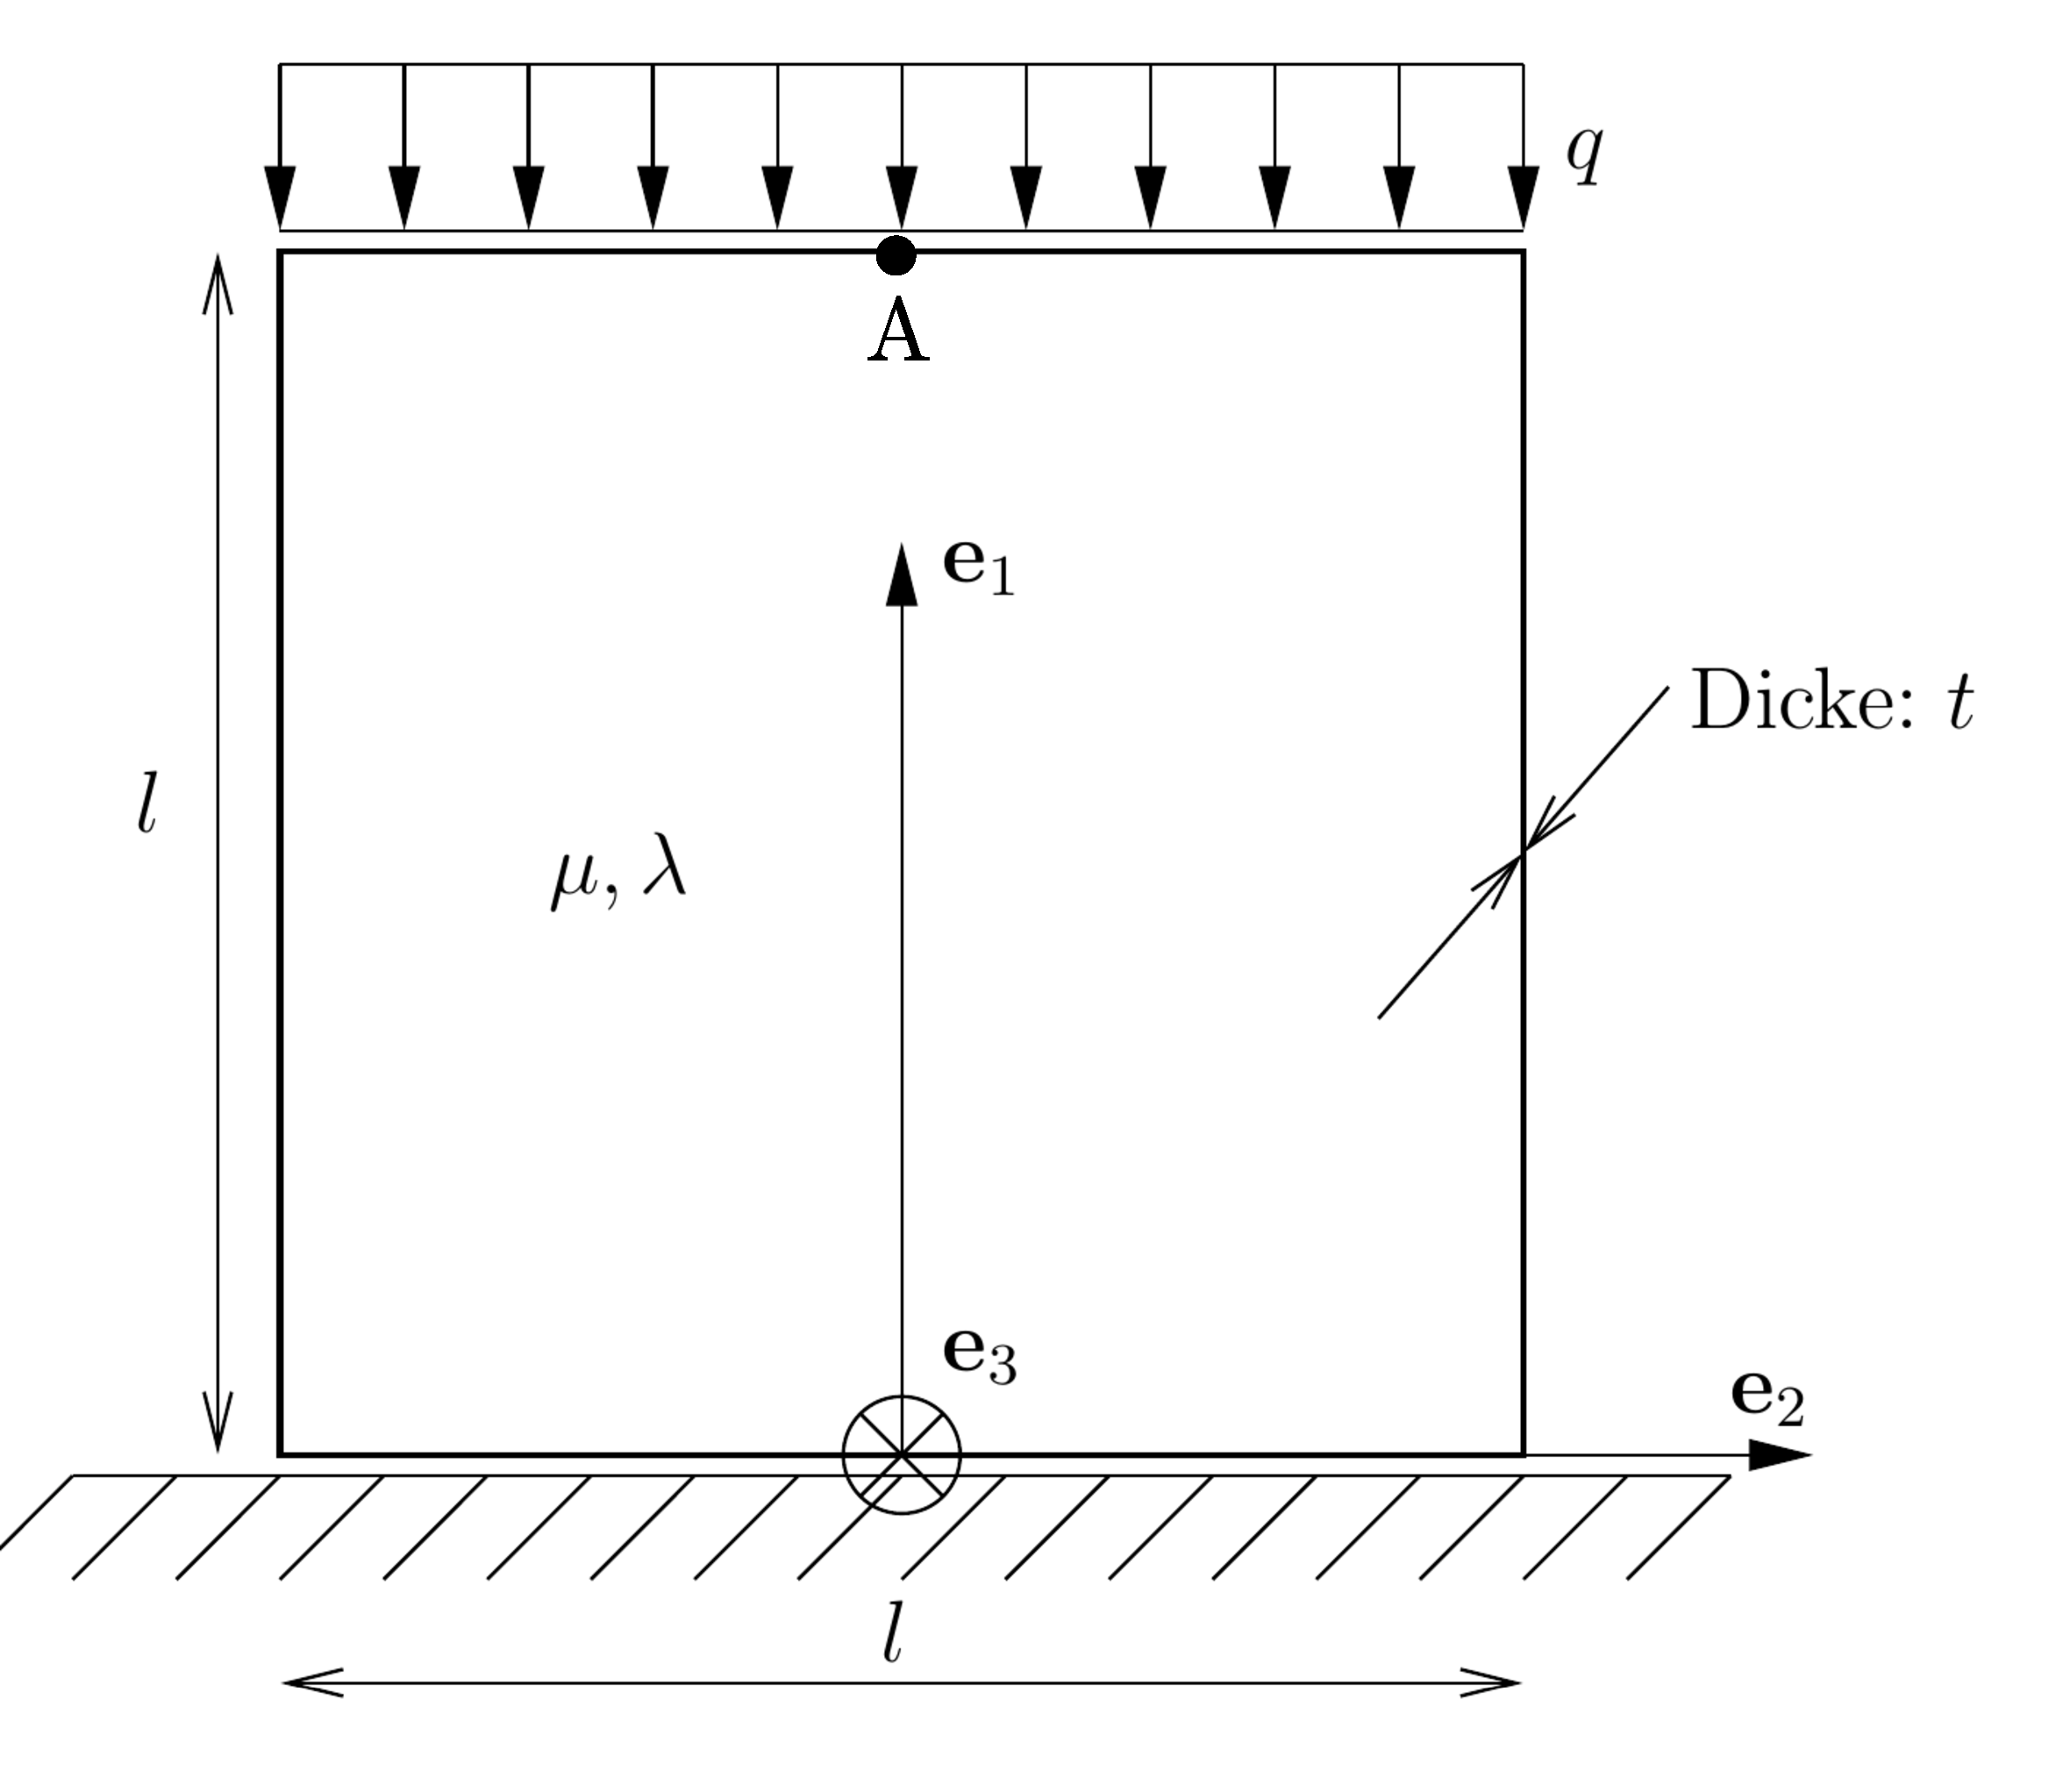
\includegraphics[width=0.6\textwidth]{fig/ue1_cube_surface_load_on_plane.pdf}
\end{center}


\enab
\item Erfüllt der Verschiebungszustand 
%$\mmu=[\alpha x_1 \,,\, \beta x_2 \,,\, \gamma x_3]^T$
$\bu= \alpha x_1 \be_1 + \beta x_2 \be_2 + \gamma x_3 \be_3$
die Impulsbilanz? 
Bestimmen Sie die Konstanten $\alpha, \beta, \gamma$ aus den Randbedingungen.
Nutzen sie dazu das Cauchy-Theorem $\Bsigma \smpc \bn=\bt$

\item Berechnen Sie die Verschiebung im Punkt A für den Parametersatz $\{E,\nu,q,t,l\}=\{210 \mrm{GPa},0.3,500 \mrm{MPa},100 \mrm{mm} ,100 \mrm{mm}\}$ 

\par \textit{Hinweis}: Die Beziehungen zwischen den Elastizitätsparametern lauten: 
\ebn \lambda=\frac{E \nu}{(1+\nu)(1-2 \nu)} \quad,\quad \mu=\frac{E}{2(1+\nu)} \een


\enae % tensorrechnung und kontinuumsmechanik

% \setcounter{section}{1}
\clearpage
\setcounter{page}{1}
\section{Variationsrechnung \label{sec:varrec}}



\subsection{Stab unter Eigengewicht}

\begin{minipage}{0.3\textwidth}
% \centering \raisebox{\dimexpr-\height+1.5ex\relax}{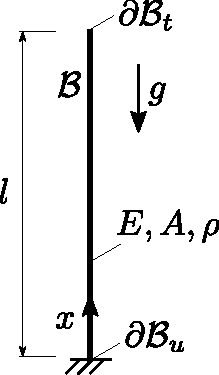
\includegraphics[scale=0.8]{fig/ue2_stab_eigengewicht.pdf}} % workarount if top alignment is needed
\center
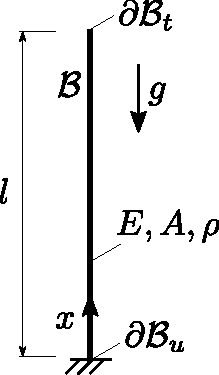
\includegraphics[scale=0.8]{fig/ue2_stab_eigengewicht.pdf}
\end{minipage}
\hfill
\begin{minipage}{0.64\textwidth}
Ein Stab ($EA=const.$) der Dichte $\rho$ und der Länge $l$ ist eingespannt an der Position $x=0$ und erfährt eine Deformation aufgrund seiner Masse im Erdschwerefeld $g$.
\enab
\item Leiten Sie mithilfe des Prinzips des Minimums des elastischen Gesamtpotentials die Euler-Lagrange Differentialgleichung für die Verschiebungsfunktion $u(x)$ her.
\item Ermitteln sie die Lösungsfunktion $u(x)$ der Differentialgleichung unter Berücksichtigung der Randbedingungen.
\enae
\end{minipage}





\subsection{Balken unter Streckenlast}

Ein Balken ($EI=const.$) der Länge $l$ erfährt eine konstante Streckenlast $q(x)=q_0$. 

\begin{center}
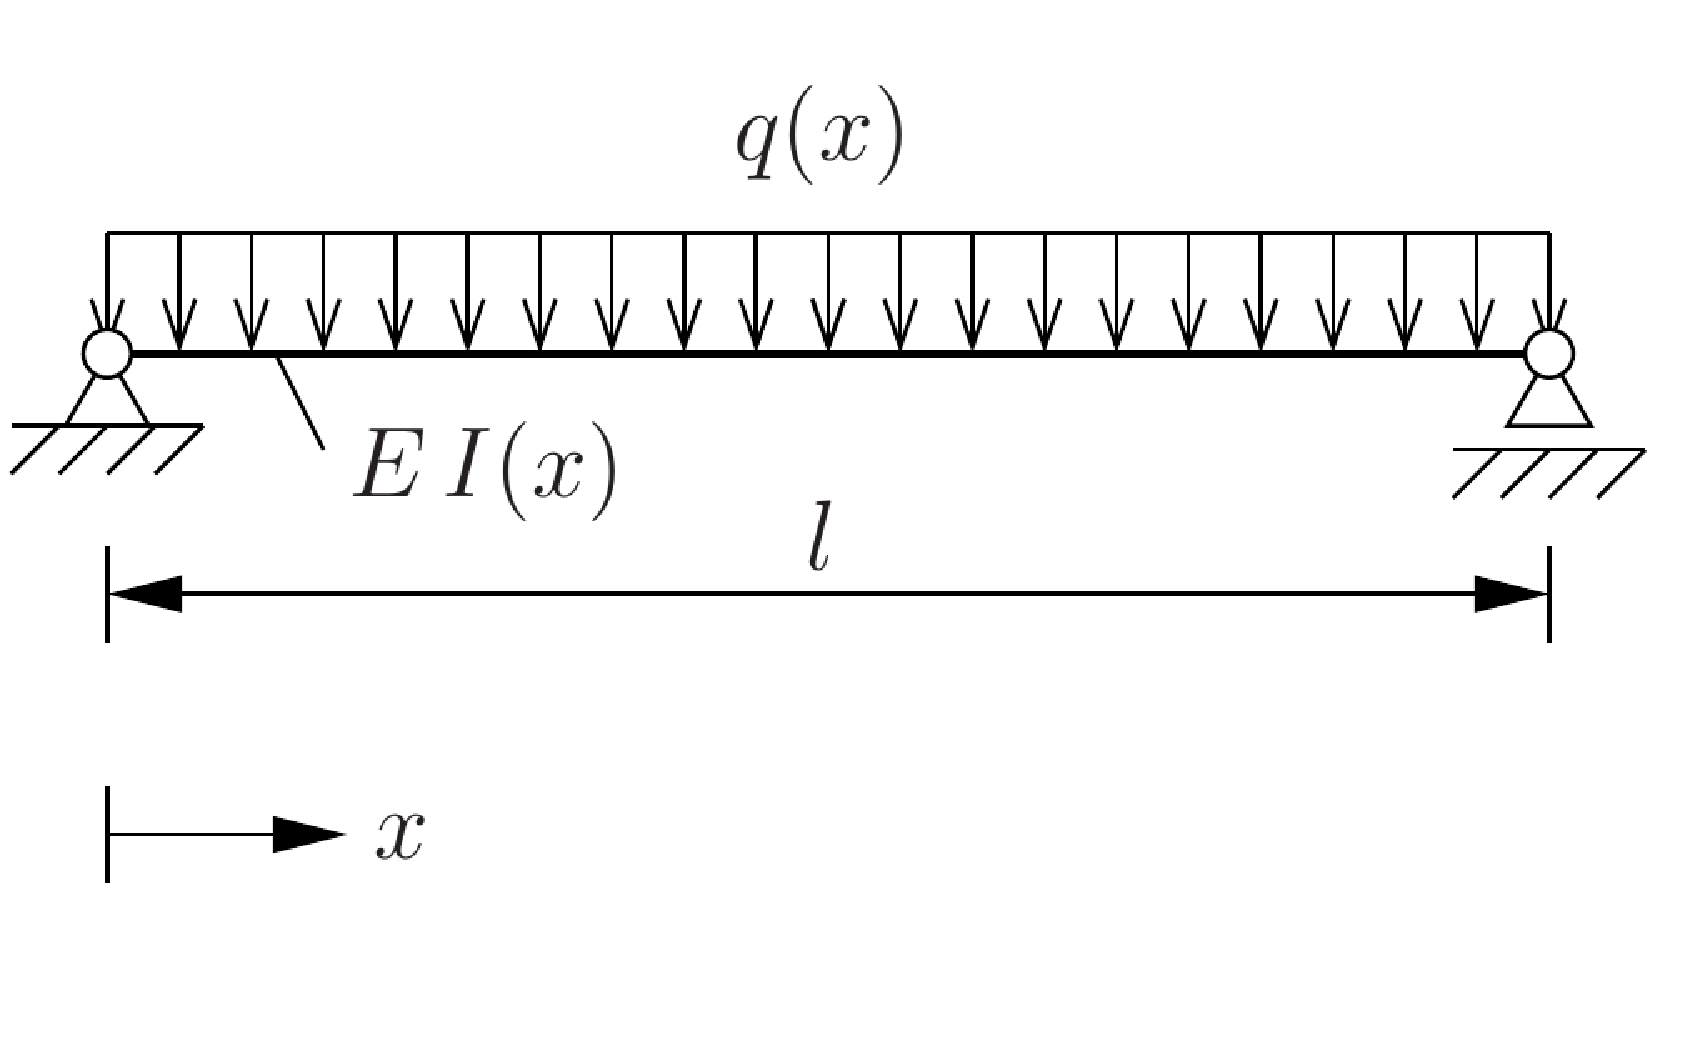
\includegraphics[width=0.44\textwidth]{fig/ue2_balken_linienlast.pdf}
\end{center}

Vorgegeben sei das folgende elastische Gesamtpotential:
%
\ebn
\Pi=\int_{0}^l \Big[ \frac{1}{2} EI(w(x)'')^2-w(x)q_0 \Big] \intd{x}
\een

\enab
\item Leiten Sie mithilfe der Variationsmethode die Euler-Lagrange Gleichung für die Durchbiegung $w(x)$ sowie die natürlichen Randbedingungen her.
\item Bestimmen sie die Biegelinie $w(x)$ unter Auswertung der Randbedingungen
\item Wie lauten die natürlichen Randbedingungen unter der Annahme, dass der Balken bei $x=0$ fest eingespannt ist und bei $x=l$ frei?
\par \textit{Hinweis}: Die essentiellen RB lauten in diesem Fall $w(0)=0$ und $w'(0)=0$.
\enae



 % variationsrechnung
% o
% % \setcounter{section}{2}
\clearpage
\setcounter{page}{1}

\section{Einführung Matlab \label{sec:einmat}}



\subsection*{Einführung}

{\bf Was ist \matl\ ?}
\begin{itemize}
\item \matl\ (abkürz. für MATrix LABoratory) ist ein Software-Paket für numerische Berechnung und Visualisierung.
Es besteht aus einer großen Anzahl an vorgefertigten Funktionen (z.B. lineare Algebra, Lösen von Differentialgleichungen, ...)

\item  Bei \matl\ steht der Fokus mehr auf numerischer Berechnung, während die Funktionalität von {\sc Maple} und {\sc Mathematica} beispielsweise mehr auf symbolische Algebera ausgerichtet ist.

\item Bekannte \matl-ähnliche Open-Source Programme: {\sc Scilab}, {\sc Octave}
\end{itemize}


{\bf Grund-Features:}
\begin{itemize}
\item Automatische Dimensionierung (d.h., keine Dimensionsangaben bei Deklaration von Vektoren und Arrays erforderlich)

\item Case-Sensitive (d.h., \verb(a( und \verb(A( sind unterschiedliche Variablen)

\item Eingebaute Funktionen basieren auf Vektor- und Matrixoperationen und sind dementsprechend auch für diese optimiert.

\item Datei-Typen:
\begin{itemize}
 \item M-Dateien: Standard ASCII Textdateien mit \verb(.m( -Dateiendung
 \item Mat-Dateien: Binärdateien, mit \verb(.mat( -Dateiendung
 \item Mex-Dateien (``\matl-Executable''): C, C++ oder Fortran Programme, welche von \matl\ aufgerufen werden können
\end{itemize}

\item Grundlegendes Daten-Objekt ist das Array, welches aus Unterelementen verschiedenster Typen (Integern, Doubles, Matrizen, Characters, Strings, Strukturen und Zellen) bestehen kann.

\item Der Typ einzelner Daten-Objekte muss nicht explizit deklariert werden. (z.B. besteht auch keine Notwendigkeit Variablen als Reel oder Komplex zu deklarieren)
\end{itemize}



\clearpage %%%%%%%%%%%%%%%%%%%%%%%%%%%%%%%%%%%%%%%%%%%%%%%%%%%%%%%%%%%%%%%%%%%%%%%%%%%
\subsection*{Grundbefehle}

\begin{tabular}{ll}
\multicolumn{2}{c}{\bf Hilfe}\\ 
\urule{2}
\verb(help <command>( & Hilfe zu \verb(<command>(\\
\verb(lookfor <string>( & listet Hilfe zu \verb(<string>( auf\\
\midrule
\end{tabular}\smallskip

\begin{tabular}{ll}
\multicolumn{2}{c}{\bf Verzeichnisbefehle}\\
\urule{2}
\verb(pwd( & aktuelles Verzeichnis anzeigen\\
\verb(cd( & Verzeichnis ändern\\
\verb(dir( / \verb(ls( & Inhalt des aktuellen Verzeichnisses anzeigen\\
\midrule
\end{tabular}\medskip

\underline{Beispiel:}

{\small\begin{verbatim}
>> help cos
 COS    Cosine.
    COS(X) is the cosine of the elements of X. 
 Overloaded methods
    help sym/cos.m
 \end{verbatim}}

 
 
\subsection*{Variablen}

\begin{tabular}{ll}
\multicolumn{2}{c}{\bf Operatoren}\\
\urule{2}
\verb(=( & einen Wert zuweisen\\
\verb(+ - * / ^( & Rechenoperatoren\\
\verb(,( (am Ende der Zeile) & Befehl mit Output\\
\verb(;( (am Ende der Zeile) & kein Output\\
\verb(...( & Zeilenumbruch innerhalb eines Befehls\\
\midrule
\end{tabular}\smallskip

\begin{tabular}{ll}
\multicolumn{2}{c}{\bf Konstanten}\\
\urule{2}
\verb(i,j( & Imaginärwert $\sqrt{-1}$\\
\verb(pi( & $\pi = 3.14\ldots$\\
\verb(inf(  & Unendlich $\inf$\\
\verb(NaN(  & not a Number, z.\ B.\ $\frac{0}{0}$\\
\verb(eps( & kleinste positive Zahl, welche sich ausgeben lässt\\
\midrule
\end{tabular}\smallskip

\begin{tabular}{ll}
\multicolumn{2}{c}{\bf Variablenmanagement}\\
\urule{2}
\verb(who( & listet die Namen aller im Workspace befindlichen Variablen auf\\
\verb(whos( & listet Namen und Größe der Variablen\\
\verb(clear( & clear Workspace\\
\verb(clear <var>( & clear Variable \verb(<var>(\\
\verb(clc( / \verb(clf( / \verb(cla( & clear command / figure / axes\\
\midrule
\end{tabular}\medskip

Für mehr Informationen: Eingabe von \verb/help +/ in \matl-Kommandozeile.\medskip

\underline{Beispiele:}\medskip

\begin{minipage}[t]{0.5\textwidth}
\small\begin{verbatim}
>> ( 47 + 1e+02 * 1.5 + 4^2 ) / 4
ans =
   53.2500
\end{verbatim}
\end{minipage}
\hfill
\begin{minipage}[t]{0.49\textwidth}
Die Variable \verb(ans( ist das Ergebnis der letzten Rechenoperation.
\end{minipage}\medskip

\begin{minipage}[t]{0.5\textwidth}
{\small\begin{verbatim}
>> a = ( 47 + 1e+02 * 1.5 + 4^2 ) / 4
a =
   53.2500
\end{verbatim}}
\end{minipage}
\hfill
\begin{minipage}[t]{0.49\textwidth}
Das Ergebnis wird in Variable \verb(a( gespeichert.
\end{minipage}

 
 
\subsection*{Mathematische Funktionen}

\begin{tabular}{ll}
\urule{2}
\verb/sqrt(x)/ & Quadratwurzel\\
\verb/xp(x)/ & Exponentialfunktion\\
\verb/log(x)/ / \verb/log10/ & Logarithmusfunktionen\\
\verb/sin(x)/ & Sinus\\
\verb/cos(x)/ & Cosinus\\
\verb/tan(x)/ & Tangens\\
\verb/atan(x)/ & Arkustangens (Winkel $-90^{\circ}\ldots+90^{\circ}$)\\
\verb/atan2(y,x)/ & Arkustangens (Winkel $-180^{\circ}\ldots+180^{\circ}$)\\
\verb/abs(x)/ & Betrag von \verb/x/\\
\verb/sign(x)/ & Signum (Vorzeichen von \verb/x/)\\
\midrule
\end{tabular}\medskip

Mehr Infos: Eingabe von \verb/help elfun/ oder
\verb/help datafun/ in \matl-Kommandozeile.\medskip


\underline{Beispiel:}\medskip

\begin{verbatim}
>> y1 = 2^2+log(pi)*sin(0.75*pi/2)+sqrt(exp(2*pi/3))
\end{verbatim}

\begin{minipage}[b]{0.5\textwidth}
\begin{verbatim}
y1 =
    7.9072
\end{verbatim}
\end{minipage}
\hfill
\begin{minipage}[b]{0.46\textwidth}
$$ y_1 = 2^2 + \ln \pi \sin(0.75\pi/2) + \sqrt{e^{2/3\pi}}$$
\end{minipage}
 
 
 
\clearpage %%%%%%%%%%%%%%%%%%%%%%%%%%%%%%%%%%%%%%%%%%%%%%%%%%%%%%%%%%%%%%%%%%%5
\subsection*{Vektoren und Matrizen}

\begin{tabular}{ll}
\multicolumn{2}{c}{\bf Vektor- und Matrixbefehle}\\
\urule{2}
\verb/[ x1 x2 ...; y1,y2,...] / & Vektor oder Matrix ('\verb/,/' oder Leerzeichen zwischen\\
 &  Spalten, '\verb/;/' oder Zeilenumbruch zwischen Reihen)\\
\verb/start: <stepsize:> end/ & Spaltenoperator (\verb/stepsize/ opt., sonst = 1)\\
\verb/linspace(start,end,num_steps)/ & linearer Zeilenvektor\\
\verb/logspace(start,end,num_steps)/ & logarithmischer Zeilenvektor\\
\verb/eye(rows,columns)/ & Einheitsmatrix [Zeilen x Spalten]\\
\verb/ones(rows,columns)/ & Matrix, bei der alle Einträge=1 sind [Zeilen x Spalten]\\
\verb/zeros(rows,columns)/ & Nullmatrix [Zeilen x Spalten]\\
\verb/rand(rows,columns)/ & Matrix mit Zufallswerten [Zeilen x Spalten]\\
\verb/a(index)/ & Element des Vektors \verb/a/ an Position \verb/index/\\
\verb/A(r,c)/ & Element der Matrix \verb/A/ an Position \verb/r/ x \verb/c/\\
\midrule
\end{tabular}\medskip

\underline{Beispiele:}\medskip

\begin{minipage}[t]{0.5\textwidth}
\small\begin{verbatim}
>> x=[1 2 3]
x =
     1     2     3
>> y=[4;5;6]
y =
     4
     5
     6
>> A=[1 2 3;4,5,6;7 8,9]
A =
     1     2     3
     4     5     6
     7     8     9
>> A(2,3)
ans =
     6
\end{verbatim}
\end{minipage}
 \hfill
\begin{minipage}[t]{0.42\textwidth}
\small\begin{verbatim}
>> A(1,2)=8
A =
     1     8     3
     4     5     6
     7     8     9
>> B=A(2:3,1:3)
B =
     4     5     6
     7     8     9
>> v=0:2:8
v =
     0     2     4     6     8
>> v=[8:-2:0]
v =
     8     6     4     2     0
\end{verbatim}
\end{minipage}


% \subsection*{Vektor- und Matrixoperationen}

\begin{tabular}{ll}
\multicolumn{2}{c}{\bf Operationen}\\
\urule{2}
\verb(.* .\ ./ .^( & elementweise Berechnung\\
\verb(\ /( & linke und rechte Division\\
\verb/transpose(A)/ oder \verb/A.'/ & Transponierte von \verb/A/\\
\verb/ctranspose(A)/ or \verb/A'/ & Transponierte von \verb/A/ (komplex Konjugiert)\\
\verb/inv(A)/ & Inverse von \verb/A/\\
\verb/det(A)/ & Determinante von \verb/A/\\
\midrule
\end{tabular}\smallskip

\begin{tabular}{ll}
\multicolumn{2}{c}{\bf Dimensionen}\\
\urule{2}
\verb/[M,N] = SIZE(A)/ & Dimension von Matrix und Vektor\\
\verb/M = SIZE(A,DIM)/ & Länge der Komponente \verb/DIM/ der Matrix \verb/A/ \\
\midrule
\end{tabular}\smallskip

\begin{tabular}{ll}
\multicolumn{2}{c}{\bf Mathematische Funktionen von Vektoren und Matrizen}\\
\urule{2}
\verb/sum(a)/ & Summe der Vektorelemente\\
\verb/prod(a)/ & Produkt der Vektorelemente\\
\verb/min(a)/ & kleinstes Vektorelement\\
\verb/max(a)/ & größtes Vektorelement\\
\verb/sort(a)/ & Elemente in aufsteigender Reihenfolge\\
\verb/find(a)/ & nicht-Null Elemente\\
\midrule
\end{tabular}\medskip

\underline{Beispiele:}\medskip

\begin{minipage}[t]{0.5\textwidth}
\small\begin{verbatim}
>> A=[1 2 3; 4 5 6; 7 8 9];
>> B=[1 2 3; 2 4 5; 3 7 8];
>> b=[2 4 6 8 10]';
>> v=0:2:8;

>> v*b
ans =
   160
>> v'*b'
ans =
     0     0     0     0     0
     4     8    12    16    20
     8    16    24    32    40
    12    24    36    48    60
    16    32    48    64    80
\end{verbatim}
\end{minipage}
\hfill
\begin{minipage}[t]{0.42\textwidth}
\small\begin{verbatim}
>> c=v+b';
>> c=v-b';
>> C=A+B;
>> C=A-B;
>> C=A*B;
>> c=A*v(1:3)'
c =
    16
    34
    52
>> c=v.*b'
c =
     0     8    24    48    80
\end{verbatim}
\end{minipage}\bigskip

\underline{Beispiel:}\medskip

\begin{minipage}[t]{0.4\textwidth}
\small\begin{verbatim}
>> A=[5 -3 2; -3 8 4; 2 4 -9];
>> b=[10;20;9];
>> x=A\b
x =
    3.4442
    3.1982
    1.1868
\end{verbatim}
\end{minipage}
\hfill
\begin{minipage}[t]{0.59\textwidth}
Lösen des linearen Gleichungssystems: $\bA\bx = \bb$
\begin{eqnarray*}
5x &=& 3y-2z+10\\
8y+4z &=& 3x+20\\
2x+4y-9z &=& 9\\
\end{eqnarray*}
\end{minipage}



\clearpage
\subsection*{Skripte und Funktionen}

\begin{itemize}
\item Skript:\\
  Wenn ein Skript aufgerufen wird, führt \matl\ schlicht die in der Datei befindlichen Befehle aus.
  Skripte können im Workspace bereits vorhandene Daten bearbeiten oder auch neue Daten erzeugen.
  Auch wenn Skriptdateien keine Outputargumente aufweisen, werden alle erzeugten Variablen im Workspace gespeichert und können in darauffolgenden Rechenoperationen verwendet werden.
\item Funktion:\\
  Funktionen sind \verb/.m/-Dateien, welche Inputargumente aufnehmen und Outputargumente wiedergeben.
  Der Name der \verb/.m/-Datei und der Funktion sollten übereinstimmen.
  Funktionen arbeiten mit lokalen Variablen in einem funktioneigenen Worskpace unabhängig des von der \matl-Kommandozeile bearbeiteten Workspaces.
\end{itemize}
Sowohl Skripte als auch Funktionen werden als .m-Datei gespeichert.\medskip

\underline{Struktur von Funktionen:}
{\small\begin{verbatim}
function [a_out,b_out] = name_of_function(a_in,b_in)
%         output list                     input list
%
% Description of function can be placed here
% by using the comment-operator '%'. This
% informations can be displyed by typing
% 'help name_of_function' at MATLAB-command-line.
.
.
a_out = a_in - a_out;
b_out = a_in + a_out;
.
.
\end{verbatim}}

\underline{Beispiel: Länge eines Vektors berechnen}
{\small\begin{verbatim}
function vlength = fvectorlength(vector)
%
% Computation of the length 'vlength' of
% a column vector 'vector'

vlength = sqrt(vector'*vector);
\end{verbatim}}
Aufrufen der Funktion:
{\small\begin{verbatim}
>> fvectorlength([-1;3;5])
ans =
    5.9161
\end{verbatim}}



\clearpage %%%%%%%%%%%%%%%%%%%%%%%%%%%%%%%%%%%%%%%%%%%%%%%%%%%%%%%%%%%%%%%%%%%%%%%%%%%%%%%%%%%%%%5
\subsection*{Logikoperatoren}

\begin{tabular}{llll}
\urule{4}
\verb(== , ~=( & gleich, nicht gleich\\
\verb(< , <=( & kleiner als, kleiner gleich\\
\verb(> , >=( & größer als, größer gleich\\
\midrule
\verb/~/ & logisches NOT & \verb/&/ & elementweise logiesches AND\\
\verb/|/ & elementweise logisches OR & \verb/xor/ & logisches EXCLUSIVE-OR\\
\midrule
\end{tabular}\medskip

Mehr Infos: Eingabe von \verb/help +/ in \matl-Kommandozeile.




\subsection*{IF-/Fallunterscheidungen und Schleifen}

\begin{tabular}{ll}
\urule{2}
\verb(IF( expression (z.B. \verb/a==1/)& IF-Statement Bedingung\\
  \hspace*{0.3cm} statements\\
\verb(ELSEIF( expression & ELSE und ELSEIF sind optional\\
  \hspace*{0.3cm} statements &  \\
\verb(ELSE(\\
  \hspace*{0.3cm} statements\\
\verb(END(\\
\midrule
\verb(SWITCH( switch-expr (z.B. \verb/id/)& SWITCH-Statement Fall \\
\verb(  CASE( case-expr, (z.B. \verb/1/) \\
  \hspace*{0.6cm} statement, ..., statement\\
\verb(  CASE {(case-expr1, case-expr2, case-expr3,...\verb(}(\\
  \hspace*{0.6cm} statement, ..., statement\\
\verb(  OTHERWISE,(\\
  \hspace*{0.6cm} statement, ..., statement\\
\verb(END(\\
\midrule
\verb(FOR( variable = expr (z.B. \verb/ii=1:10/)& Wiederholung der Statements\\
  \hspace*{0.3cm} statement, ..., statement & in einer spezifischen Anzahl.\\
\verb(END(\\
\midrule
\verb(WHILE( expression (z.B. \verb/ii<imax/)& Wiederholung der Statements eine  \\
  \hspace*{0.3cm} statements & unbestimmte Anzahl bis Bedingnung erfüllt.\\
\verb(END(\\
\midrule
\end{tabular}



\clearpage %%%%%%%%%%%%%%%%%%%%%%%%%%%%%%%%%%%%%%%%%%%%%%%%%%%%%%%%%%%%%%%%%%%%%%%%%%%%%
\subsection*{Plotten von Schaubildern}

\begin{tabular}{ll}
\multicolumn{2}{c}{\bf Bedienen des 'figure'-Fensters}\\
\urule{2}
\verb/figure , figure(no)/ & erstellen, aktivieren eines Schaubilds mit Nummer \verb/no/\\
\verb/subplot(num_rows,num_cols,index)/ & erstellen eines Subplots\\
& z.B., \verb/subplot(2,3,2)/: Subplot mit 2 Zeilen\\
& und 3 Spalten, aktivieren eines 2. Subplots\\
\verb/gcf/ & 'get current figure'\\
\verb/clf/ & 'clear active figure'\\
\verb/delete(id)/ & Objekte mit \verb(id( löschen\\
\verb/close(index)/ & 'figure'-Fenster Nr. \verb(index( löschen\\
\verb/close all /& alle 'figure'-Fenster löschen\\
\verb/hold <on | off>/ & aktuelles 'figure'-Fenster geöffnet lassen\\
& bei Generierung neuer Plots an/aus \\
\midrule
\end{tabular}\smallskip

\begin{tabular}{ll}
\multicolumn{2}{c}{\bf 2-D Plot Befehle}\\
\urule{2}
\verb/plot(<x,>y<,plotstyle>/,...) & Plot, Linear (\verb/<>/ = opt.)\\
\verb/fplot(func,range)/ & Plot einer expliziten Funktion\\
\verb/line(x,y)/ & erstellen der Linie durch Koordinatenvektoren \verb/x,y/\\
\verb/text(x,y,string)/ & platzieren von \verb/string/ an Position \verb/x,y/\\ 
\multicolumn{2}{l}{Für mehr Infos über 2-D Plots: aufrufen von {\ttfamily help plot} in Kommandozeile.}\\
\midrule
\end{tabular}\smallskip

\begin{tabular}{ll}
\multicolumn{2}{c}{\bf 3-D Plot Befehle}\\
\urule{2}
\verb/plot3(x,y,z <,plotstyle> ,...)/ & dreidimensionaler Plot\\
\verb/sphere/ & plotten einer Kugel\\
\verb/[x,y,z] = sphere/ & Koordinaten einer Einheitskugel unter \verb/x,y,z/ speichern\\
\verb/line(x,y,z)/ & erstellen einer Linie durch Koordinatenvektoren \verb/x,y,z/\\
\verb/text(x,y,z,string)/ & platzieren von \verb/string/ an Position \verb/x,y,z/\\
\midrule
\end{tabular}\smallskip

\begin{tabular}{lll|lll}
\multicolumn{6}{c}{\bf Plotstyles}\\
\urule{6}
\multicolumn{3}{c}{Farben:} & \multicolumn{3}{c}{Linienstyles:}\\
\verb/k/ schwarz & \verb/r/ rot & \verb/g/ grün & 
\verb/-/ durchgängig    & \verb\o\ Kreis & \verb/./ Punkte\\
\verb/b/ blau  & \verb/m/ magenta & \verb/w/ weiß &
\verb/--/ gestrichelt  & \verb\*\ sterne & \verb\x\ x\\
\verb/c/ cyan  & \verb/y/ gelb & &
\verb/:/ gepunktet   & \verb\+\ plut & \verb/-./ Punkt-Strichlinie\\
Mehr Infos: \verb/help plot/\\
\midrule
\end{tabular}\bigskip

\begin{minipage}[c]{0.54\textwidth}
\underline{Beispiele:}
\small\begin{verbatim}
>> figure(1)
>> clf
>> t=0:pi/20:2*pi;
>> plot(t,sin(t),'-.r*')
>> hold on
>> plot(t,(sin(t-pi/2)),'linestyle','--',...
   'marker','o','color','m')
>> plot(t,sin(t-pi),':bs')
>> hold off
\end{verbatim}
\end{minipage}
\hfill
\begin{minipage}[c]{0.45\textwidth}
\centering
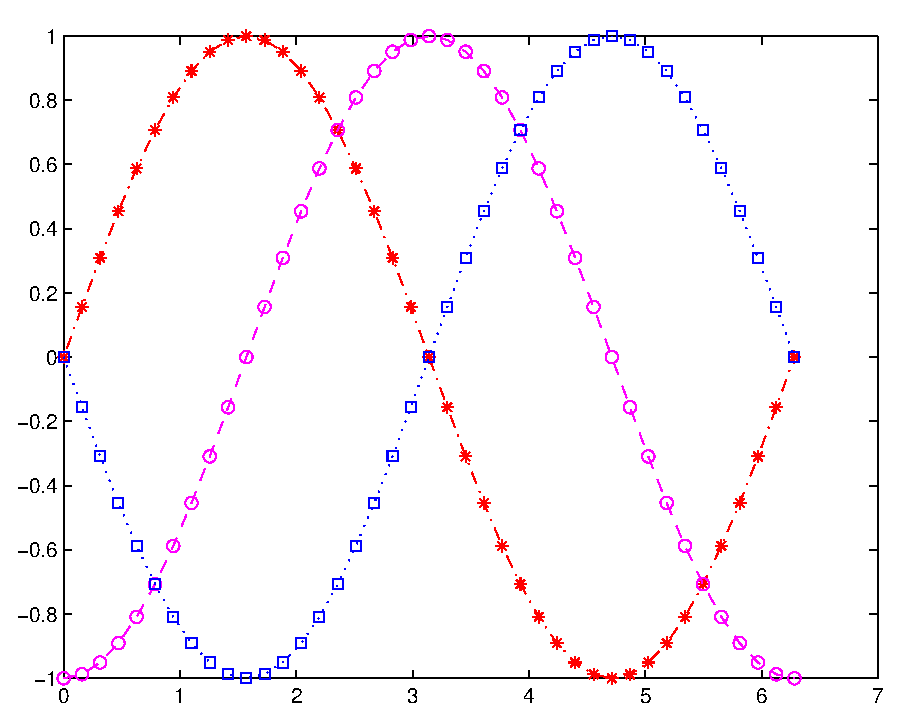
\includegraphics[width=0.8\textwidth]{fig/ue3_plot_example.eps}
\end{minipage}\bigskip

\begin{tabular}{ll}
\multicolumn{2}{c}{\bf Labeln von Achsen und Figures}\\
\urule{2}
\verb/axis([xmin,xmax,ymin,ymax<,zmin,zmax>)/ & Skalierung (min=\verb/-inf/ oder\\
& max=\verb/inf/ $\rightarrow$ Auto Skalierung) \\
\verb/axis <on | off | auto | equal | square>/ & verschiedene Achsen-Befehle\\
& Mehr: \verb/help axis/\\
\verb/grid <on | off>/ & Gitter an/aus\\
\verb/gca/ & Wiedergabe der aktuellen Achse\\
\verb/cla/ & löschen der aktuellen Achse\\
\verb/xlabel(string)/ & Label der x-Achse\\
\verb/ylabel(string)/ & Label der y-Achse\\
\verb/zlabel(string)/ & Label der z-Achse\\
\verb/title(string)/ & Titel der aktuellen Achse\\
\verb/legend(string_1,string_2,...<,pos>)/ & Legende platzieren\\
& \verb/pos = 0,1,2,3,4,-1/\\
\midrule
\end{tabular}



\clearpage %%%%%%%%%%%%%%%%%%%%%%%%%%%%%%%%%%%%%%%%%%%%%%%%%%%%%%%%%%%%%%%%%%%%%%%%%%%%%%%%%%%%%%%%%%%%%
\subsection{Animation eines rotierenden Kragarms}

\begin{minipage}[t]{0.5\textwidth}
Ein Kragarm der Länge $L$ ist am oberen Ende (Punkt P2) an einer vertikalen Stange (höhe H) befestigt.
Der Kragarm ist im Winkel $\alpha$ zur Stange geneigt.
Die Stange ist am unteren Ende (Punkt P1) drehbar gelagert mit der $z$-Achse als Rotationsachse.
Am Freien Ende des Kragarms (Punkt P3) ist eine Kugel mit dem Radius $R$ befestigt.\smallskip

Programmieren Sie ein \matl-Skript (\verb/.m/-file), in welchem die Rotation $\varphi$ um die $z$-Achse des dargestellten Systems in animierter Form dargestellt wird.
\end{minipage}
\hfill
\begin{minipage}[t]{0.39\textwidth}
\begin{picture}(0,0)
\unitlength1cm
% \includegraphics{fig/bild1020.pdf}
 \put(0.0,-5.0){\scalebox{0.8}{\input{fig/ue3_bild1020.pdf_t}}}
\end{picture}
\end{minipage}\bigskip

\textit{Hinweis:} Nutzen sie die Rotationsmatrix 

\ebn
 \bR =
 \begin{bmatrix}
       \cos{\varphi} & -\sin{\varphi} &     0 \\
       \sin{\varphi} & \cos{\varphi}  &     0 \\
        0            &      0         &     1
 \end{bmatrix},
\een

welche mit $\bar{\bv}=\bR \smpc \bv$ die Rotation eines Vektors $\bv$ um die $z$-Achse beschreibt.

\subsection{Animation mithilfe einer Subroutine}

Das \matl-Skript aus der vorherigen Aufgabe soll nun modifiziert werden.
Eine selbst programmierte Funktion soll die rotierten Koordinaten für die Animation berechnen.
Input parameter sollen die die Ursprungskoordinaten und der Rotationswinkel $\varphi$ sein.
Der Output der Funktion sollten die Koordinaten des rotierten Systems sein.
 % einfüzhrung matlab
% % \setcounter{section}{3}
% \clearpage
\section*{\matl-Code Demonstrations}

\subsection*{Subroutine \tt PlaneTrussElementStiffness.m}

\input{tex/code_tex/ue5/t_PlaneTrussElementStiffness.m}



\subsection*{Hauptdatei \tt PlaneTruss.m}

\input{tex/code_tex/ue5/t_PlaneTruss.m}



\subsection*{Subroutine \tt PlaneTrussAssemble.m}

\input{tex/code_tex/ue5/t_PlaneTrussAssemble.m}

\subsection*{\tt Assemble1.m}

\input{tex/code_tex/ue5/t_Assemble1.m}

\subsection*{\tt Assemble2.m}

\input{tex/code_tex/ue5/t_Assemble2.m}

\subsection*{\tt Assemble3.m}

\input{tex/code_tex/ue5/t_Assemble3.m}

\subsection*{\tt Assemble4.m}

\input{tex/code_tex/ue5/t_Assemble4.m}



% \textbf{fsolvelineqs.m}
% 
% \input{tex/ue3_demo/t_fsolvelineqs.m}
% 
% 
% \subsection*{Plot 2D: $\boldsymbol{\mrm{plt}\_\mrm{trig}\_}$demo.m}
% 
% \input{tex/ue3_demo/t_plt_trig_demo.m}
% 
% 
% 
% \subsection*{Solution: $\boldsymbol{\mrm{t}\_\mrm{rotating}\_\mrm{cantilever}}$.m}
% 
% \input{tex/ue3_demo/t_rotating_cantilever.m}
% 
% 
% 
% \subsection*{Solution: $\boldsymbol{\mrm{t}\_\mrm{rotating}\_\mrm{cantilever}\_\mrm{with}\_\mrm{function}}$.m}
% 
% \input{tex/ue3_demo/t_rotating_cantilever_with_function.m}
% 
% $\boldsymbol{\mrm{t}\_\mrm{frotation}\_\mrm{z}.\mrm{m}}$
% 
% \input{tex/ue3_demo/t_frotation_z.m}




% 
% % \setcounter{section}{3}
\clearpage
\setcounter{page}{1}

\section{Assemblierung}


\subsection{Ebenes Fachwerk\label{subsec:assfw1}}

Gegeben sei das folgende Fachwerk:\medskip

\begin{minipage}[b]{0.4\textwidth}
  \input{fig/ue4_fachwerk1.pdf_tex}
  \captionof{figure}{Randwertproblem}
  \label{fig:fachw1}
\end{minipage}
 \hfill
\begin{minipage}[b]{0.56\textwidth}
  \input{fig/ue4_fachwerk1_diskret.pdf_tex}
  \captionof{figure}{Element- und Knotennummerierung}
  \label{fig:fw1dis}
 \end{minipage}
 



\enab
\item Welche grundlegenden Schritte sind erforderlich um das Problem mithilfe der Finite-Elemente Methode zu lösen?
\enae

Im Folgenden sei angenommen, dass die jeweiligen Elementsteifigkeitsmatrizen $\mk^e$ bekannt sind.

\enabres
\item Assemblieren Sie aus den Elementsteifigkeitsmatrizen die globale Steifigkeitsmatrix $\mK$ unter Berücksichtigung der Dirichlet-Randbedingungen. 
 Stellen Sie den globalen Lastvektor $\mP$ und das globale Gleichungssystem auf.
%(Was würde mit der resultierenden globalen Steifigkeitsmatrix passieren wenn diese nicht berücksichtigt werden würden?)
\enae

Nutzen Sie die in Abbildung \ref{fig:fw1dis} dargestellte Element- und Knotennummerierung. 





\subsection{Ebenes Fachwerk}

Gegeben sei das dargestellte ebene Fachwerk, für das die jeweiligen Elementsteifigkeitsmatrizen $\mk^e$ als bekannt angenommen werden.\medskip


\begin{minipage}[b]{0.44\textwidth}
  \input{fig/ue4_fachwerk2.pdf_tex}
  \captionof{figure}{Randwertproblem}
  \label{fig:fachw2}
\end{minipage}
\hfill
\begin{minipage}[b]{0.5\textwidth}
   \input{fig/ue4_fachwerk2_diskret.pdf_tex}
  \captionof{figure}{Diskretisierung}
  \label{fig:fw2dis}
 \end{minipage}\medskip

Stellen Sie den globalen Lastvektor und die globale Steifigkeitsmatrix unter Berücksichtigung der Dirichlet-Randbedingungen auf.
Nutzen Sie die vorgegebene Diskretisierung.
 % assemblierung
% 
%  \setcounter{section}{4}
\clearpage
\setcounter{page}{1}

\section{FEM mit Stabelementen}



\subsection{Elementsteifigkeitsmatrix\label{subsec:stabke}}

Betrachtet wird das Fachwerk aus Aufgabe 4.1.\medskip

\begin{minipage}[b]{0.4\textwidth}
  \input{fig/ue5_fachwerk1.pdf_tex}
%   \captionof{figure}{}
%   \label{fig:fachw1}
\end{minipage}
 \hfill
\begin{minipage}[b]{0.56\textwidth}
  \input{fig/ue4_fachwerk1_diskret.pdf_tex}
%   \captionof{figure}{Element- und Knotennummerierung}
%   \label{fig:fw1dis}
 \end{minipage}
 
\enab
 \item Wie lassen sich die Einträge der Elementsteifigkeitsmatrizen $\mk^e$ berechnen? \\
   Werten Sie auch die Spezialfälle $\alpha\in\{\pi / 2, 3\pi /2\} $ und $\alpha\in\{0,\pi\}$ aus.
 \item Schreiben Sie die \matl-Funktion {\tt PlaneTrussElementStiffness.m} zur Berechnung der Elementsteifigkeitsmatrizen. 
   Verwenden sie die Parameter aus Tabelle \ref{tab:inppte}
\enae

\textit{Hinweis:}
$\tt PlaneTrussElementStiffness.m$ ist eine Subroutine zur Berechnung der Elementsteifigkeitsmatrix im globalen Koordinatensystem.
Die Inputwerte sind E-Modul $\tt E$, Stabquerschnitt $\tt A$ und die Knotenkoordinaten $\tt i$ und $\tt j$ (vgl. Abbildung \ref{fig:ten083}).
\begin{verbatim} 
  node_i(1) = x(1) 
  node_i(2) = y(1)  
  node_j(1) = x(2) 
  node_j(2) = y(2)  
\end{verbatim} 

Outputgröße ist die Elementsteifigkeitsmatrix im globalen x,y-Koordinatensystem:
  \ebn
  \mk^\mrm{e} = \mT^T \; \tilde{\mk} {}^\mrm{e} \; \underline \bT
  \quad \text{mit} \quad 
  \tilde{\mk} {}^\mrm{e} = \int_{\B^\mrm{e}} (\mB^\mrm{e})^T EA \; \mB^{\mrm{e}} \; \mrm{d} \tilde{x }
  \een
%\medskip

\begin{minipage}[b]{0.46\textwidth}
   \scalebox{0.8}{\input{fig/ue5_ten083.pdf_t}}
%   \setlength{\baselineskip}{11pt} 
  \captionof{figure}{}%Knotenkoordinaten in {\tt PlaneTrussElementStiffness.m}}
  \label{fig:ten083}
\end{minipage}
 \hfill
%  \begin{figure}[htb] \unitlength 1 cm
\begin{minipage}[b]{0.46\textwidth}
 \begin{tabular}{ll}
  \multicolumn{2}{c}{Inputparameter}\\
\toprule
\tt E & {\tt 10000} $\mrm{kN}/\mrm{m}^2$\\
\tt A & {\tt 0.02} $\mrm{m}^2$ \\
\tt node no.1: [ x y ] & \tt [ 0 0 ] $\mrm{m}$ \\
\tt node no.2: [ x y ] & \tt [ 1 2 ] $\mrm{m}$ \\
\tt node no.4: [ x y ] & \tt [ 3 2 ] $\mrm{m}$ \\
\midrule
\end{tabular}
\captionof{table}{}
\label{tab:inppte}
 \end{minipage}\medskip
%  \end{figure}

\enabres
 \item Bestimmen Sie den Lösungsvektor $\mD$ mithilfe des in der vorherigen Übung aufgestellten globalen Gleichungssystems. 
 Die Kräfte betragen $F_x = 0.01\,\mrm{kN}$ und $F_y = -0.05\, \mrm{kN}$.
\enae




\subsection{Schreiben eines FEM-Programms}

Im Folgenden soll ein eigener FE-Code in \matl\ erzeugt werden, mithilfe dessen die Knotenverschiebungen von ebenen Fachwerken berechnet werden können.
Der Workflow des Programms kann Abbildung \ref{fig:workfl} entnommen werden.
Dabei stellt die Datei $\tt PlaneTruss.m$ die Hauptdatei dar. 
Mit ihr werden zunächst Element- und Knotendaten des Fachwerkes eingelesen.
Daraufhin werden mithilfe der Subroutinen $\tt PlaneTrussElementStiffness.m$ und $\tt PlaneTrussAssemble.m$ die Elementsteifigkeitsmatrizen aufgestellt und im globalen Gleichungssystem assembliert.
Schließlich wird der globale Lastvektor aufgestellt und das globale Gleichungssystem gelöst.\medskip

% programmcode workflow
%----------------------------------------
\begin{figure}[htb]
\unitlength1cm
\fboxsep2mm
\begin{picture}(15,15)(0,-14.5)
  \put(7.5,  0){\vector(0,-1){1}}
  \put(7.5,  0){\makebox[0mm]{\fcolorbox{black}{white}{read general properties}}}
  \put(7.5, -1.5){\vector(0,-1){1}}
  \put(7.5, -1.5){\makebox[0mm]{\fcolorbox{black}{white}{nodes, coordinates and stiffnes ($E$ and $A$)}}}
  \put(7.5, -3){\vector(0,-1){1}}
  \put(7.5, -3){\makebox[0mm]{\fcolorbox{black}{white}{compute number of equations}}}
  \put(7.5, -4.5){\vector(0,-1){1.0}}
  \put(7.5, -5.5){\circle*{0.1}}
  \put(7.5, -5.5){\vector(0,-1){0.75}}
  \put(7.5, -4.5){\makebox[0mm]{\fcolorbox{black}{white}{complete assemble matrix}}}
  \put(7.5, -6.75){\vector(0,-1){1}}
  \put(7.5, -6.75){\makebox[0mm]{\fcolorbox{black}{white}{compute local element stiffness $\underline \bk^e$}}}
  \put(11, -6.75){$\rightarrow$ \tt PlaneTrussElementStiffness.m}
  \put(7.5, -8.65){\vector(0,-1){1.5}}
  \put(7.5,-10.15){\circle*{0.1}}
  \put(7.5,-10.15){\vector(0,-1){0.75}}
  \put(7.5, -8.65){\makebox[0mm]{\fcolorbox{black}{white}{assemble global stiffness matrix
$\underline \bK = \Assem \; \underline \bk^e $}}}
  \put(12, -8.65){$\rightarrow$ \tt PlaneTrussAssemble.m}
  \put(7.5,-11.4){\vector(0,-1){1}}
  \put(7.5,-11.4){\makebox[0mm]{\fcolorbox{black}{white}{complete global force vector (interactive)}}}
  \put(7.5,-12.9){\vector(0,-1){1}}
  \put(7.5,-12.9){\makebox[0mm]{\fcolorbox{black}{white}{solve system of equations to compute displacements}}}
  \put(7.5,-14.4){\makebox[0mm]{\fcolorbox{black}{white}{postprocess (print data)}}}
  
  \put(2.5, -5.5){\vector(1,0){5}}
  \put(2.5, -5.5){\line(0,-1){4.65}}
  \put(2.5,-10.15){\line(1,0){5}}

  \put(7.7,-5.6){begin loop over elements $e$}
  \put(7.7,-10.25){end loop if $e > nele$}

\end{picture}\medskip
\caption{Workflow von $\tt PlaneTruss.m$ }
\label{fig:workfl}
\end{figure}

% inputdata
%-----------------------------------------------
\clearpage
\enab
 \item Erzeugen sie zunächst in der Hauptdatei {\tt PlaneTruss.m} ein Interface, mit welchem die Element- und Knotendaten sowie die Dirichlet-Randbedingungen eingelesen werden.
\enae

\textit{Hinweis:} 
Anhand des einfachen Fachwerks in Abbildung \ref{fig:ten086} soll veranschaulicht werden wie die entsprechenden Daten eingelesen und abgespeichert werden.

\begin{figure}[htb] \unitlength 1 cm
\begin{picture}(14,4.0)%
 \put(0.0,-0.3){\scalebox{0.8}{\input{fig/ue5_ten086.pdf_t}}}
 \put(6.4,0.3){\scalebox{0.8}{\input{fig/ue5_ten087.pdf_t}}}
\put(0.0,0.0){a)}
\put(6.4,0.0){b)}
\end{picture}
% \setlength{\baselineskip}{11pt} 
\medskip
\caption{Fachwerk: 
a) Dimension (in Metern) und Randbedingungen,
b) Diskretisierung.}
\label{fig:ten086}
\end{figure}

Nach dem Programmstart soll zunächst folgender Input erfolgen:

{\small 
\begin{verbatim}
>> PlaneTruss
give the total number of elements. num_ele = 2
give the total number of nodes.  num_nodes = 3
\end{verbatim}}

Im nächsten Schritt wird die Matrix $\tt connectivity$ erstellt.
In ihr wird abgespeichert, welche globale Knotennummer zu welchem element gehört. 
Sie hat die Dimension $ \left[\, \tt nodes\_ele \times \tt num\_ele\, \right] $, wobei $\tt nodes\_ele=2$ die Anzahl der Knoten je Element darstellt.
In diesem Beispiel besitzt Element 1 die globalen Knoten 1 und 2; Element 2 hat die Knoten 2 und 3.
Die $\tt connectivity$-Matrix sieht wie folgt aus:

\ebn
\tt
connectivity = \begin{bmatrix}
                  1 & 2 \\
                  2 & 3
                 \end{bmatrix}
\label{eq:conne1}
\een

Der E-Modul sei mit 
$
 \rm
 E = 10 000 \, kN/m^2
 $
festgelegt und die Querschnittsfläche der Elemente 1 und 2 sei
\ebn
 \rm
 0.02 \, m^2 \quad und \quad 0.015 \, m^2.
 \een
 
Die Elementdaten werden nun wie folgt eingegeben

{\small 
\begin{verbatim}
element no.1
  global node for 1st local node = 1
  global node for 2nd local node = 2
  element data           [ E A ] = [10000 0.02]
 
element no.2
  global node for 1st local node = 2
  global node for 2nd local node = 3
  element data           [ E A ] = [10000 0.015],
\end{verbatim}}

wobei die eingegebenen Knotennummern in der $\tt connectivity$-Matrix gespeichert werden.\medskip

Nun werden für alle Knoten die ($\rm x,y$)-Koordinaten eingegeben
Die entsprechende $\tt X$-Matrix der Knotenkoordinaten  der Dimension  $ \left[\, \tt dof\_nodes \times \tt num\_nodes\, \right] $ lautet:

\ebn
\tt
X = \begin{bmatrix}
                  0 & 2 & 4\\
                  0 & 2 & 2
                 \end{bmatrix}
\label{eq:Xmatr1}
\een

Der Input sieht wie folgt aus:

 
{\small 
\begin{verbatim}
node no.1
  global node coordinates [ x y ] = [0 0]
 
node no.2
  global node coordinates [ x y ] = [2 2]
 
node no.3
  global node coordinates [ x y ] = [4 2]
\end{verbatim}}
 
Die Anzahl an Dirichlet-Randbedingungen $\tt num\_bc$ beträgt 4. 
Nach der Eingabe 
\begin{verbatim}
 give the total number of displacement boundary conditions
                                        num_bc = 4
\end{verbatim}


kann nun die Anzahl an verbleibenden Freiheitsgraden mit
\eb
\tt num\_eq= num\_nodes * dof\_nodes - num\_bc
\label{eq:numeq}
\ee 
bestimmt werden.
Die Horizontal- und Vertikalverschiebungen der Knoten 1 und 3 werden auf Null gesetzt:
\ebn
\rm
d^{\nodeid 1}_1 = d^{\nodeid 1}_2 = d^{\nodeid 3}_1 = d^{\nodeid 3}_2 = 0,
\een 
bzw.
\ebn
\rm
D_1 = D_2 = D_5 = D_6 = 0.
\een 

Im Zusammenhang mit diesem Schritt wird die Matrix $\tt assembleid$ erstellt. 
Sie hat die Dimension $ \left[\, \tt dof\_nodes \times \tt num\_nodes\, \right] $ und beinhaltet alle verbleibenden Freiheitsgrade.
An den Positionen, an denen Dirichlet-Randbedingungen vorliegen, befinden sich Nulleinträge. 
Für das Beispiel lautet sie also:

\ebn
\tt
assembleid = \begin{bmatrix}
                  0 & 1 & 0\\
                  0 & 2 & 0
                 \end{bmatrix}
\label{eq:asmat1}
\een


Die Inputsequenz dazu lautet:
{\small 
\begin{verbatim}
    input of global dofs with zero boundary displacements
                                   for i from 1 to num_bc
        global node of constrained degree of freedom = 1
          degree of freedom to constrained (1=x,2=y) = 1
        global node of constrained degree of freedom = 1
          degree of freedom to constrained (1=x,2=y) = 2
        global node of constrained degree of freedom = 3
          degree of freedom to constrained (1=x,2=y) = 1
        global node of constrained degree of freedom = 3
          degree of freedom to constrained (1=x,2=y) = 2
\end{verbatim}}



% assemblierung
%-----------------------------------------------
\enabres
\item Setzen Sie die Assemblierung der Elementsteifigkeitsmatrizen zur globalen Steifigkeitsmatrix algorithmisch in Form von \matl\ Code in der Hauptdatei $\tt PlaneTruss.m$ und mithilfe der Subroutinen $\tt PlaneTrussElementStiffness.m$ und $\tt PlaneTrussAssemble.m$ um.
\enae

\textit{Hinweis:}
Die Assemblierung findet in einer Schleife über die Elemente statt, in der für jedes Element zunächst die lokale Steifigkeitsmatrix $\mk^e$ (mithilfe von $\tt PlaneTrussElementStiffness.m$) erzeugt wird.
Mithilfe der Subroutine $\tt PlaneTrussAssemble.m$ soll die globale Steifigkeitsmatrix nun an den passenden Einträgen mit den jeweiligen Einträgen der lokalen Steifigkeitsmatrix besetzt werden. 
Um diesen Prozess zu veranschaulichen wird das Fachwerk in Abbildung \ref{fig:ten078} betrachtet

\begin{figure}[htb] \unitlength 1 cm
\begin{picture}(14,3.0)%
\put(0.5,0){\scalebox{0.8}{\input{fig/ue5_ten078.pdf_t}}}
\end{picture}
\setlength{\baselineskip}{11pt} 
\caption{}
\label{fig:ten078}
\end{figure}

Die $\tt connectivity$-Matrix lautet:

\ebn
\tt
connectivity = \begin{bmatrix}
                 1 & 3 & 1 & 2 & 3 & 4 & 5 & 2 & 4 \\
                 3 & 5 & 2 & 3 & 4 & 5 & 6 & 4 & 6
                 \end{bmatrix}
\een

Das Randwertproblem besteht aus neun Stabelementen, sechs Knoten und vier essentiellen Randbedingungen, d.h. 
 \ebn 
\tt num\_ele = 9  ,\quad num\_nodes = 6  ,  \quad num\_bc = 4  .
\een

Die Elementsteifigkeitsmatrix $\bk^e$ hat die Dimension $\left[\,\tt k^e_{dim} \times k^e_{dim} \right]$ mit

\ebn
\tt k^e_{dim}=nodes\_ele * dof\_nodes = 4.
\een

Die Dimension der globalen Steifigkeitsmatrix $\mK$ unter Berücksichtigung der Dirichlet Randbedingungen ist  $\left[\,\tt num\_eq \times num\_eq \right]$ mit $\tt num\_eq=8$ \eqref{eq:numeq}.
Die $\tt assembleid$-Matrix lautet

\ebn
\tt
assembleid = \begin{bmatrix}
                  1 & 2 & 4 & 6 & 8 & 0\\
                  0 & 3 & 5 & 7 & 0 & 0
                 \end{bmatrix}.
\een

Mit ihrer Hilfe werden die einzelnen Einträge $[\bk^e]_{\mrm{ij}}$ der Elementsteifigkeitsmatrix den Einträgen $[\bK]_{\mrm{IJ}}$ der globalen Steifigkeitsmatrix zugeordnet.
Bevor dies geschieht wird jedoch zunächst die leere globale Steifigkeitsmatrix aufgestellt mit 

\ebn
\rm
K_{IJ} = 0.0 \quad \text{für} \quad I,J = 1,...8 \;.
\een

Nun wird der Element-Schleifendurchlauf gestartet.
In jedem Iterationsschrit wird zunächst die lokale Elementsteifigkeitsmatrix $\mk^e$ mit $\tt PlaneTrussElementStiffness.m$ erzeugt.
Daraufhin wird mithilfe der Subroutine $\tt PlaneTrussAssemble.m$ die globale Steifigkeitsmatrix $\mK$ geupdatet.
Um diesen Vorgang zu verdeutlichen wird der erste Iterationsschritt (Element $e=1$) betrachtet. 
Die Positionen $\mrm{I}$ und $\mrm{J}$ in der globalen Matrix können den Einträgen der $\tt connectivity$- und $\tt assembleid$- Matrix entnommen werden:
%
\begin{align*}
 \mrm{I} &= \tt assembleid(:,connectivity(1,1))= [\ 1\ \ 0\ ]  \\
 \mrm{J} &= \tt assembleid(:,connectivity(1,2))= [\ 4\ \ 5\  ]
\end{align*}
%
mit der Elementsteifigkeitsmatrix

\ebn
\rm
\renewcommand{\arraystretch}{1.5}
\begin{array}{rrccccl|l}
 & & 1 & 0 & 4 & 5 & & \mbox{global dof}\\\cline{2-8}
%
& \multirow{4}{2mm}{$\renewcommand{\arraycolsep}{0mm}\left[\begin{array}{r}
\phantom{1}\\\phantom{1}\\\phantom{1}\\\phantom{1}
\end{array}\right.$}
& \rm k^{\elemid 1}_{11} & \rm k^{\elemid 1}_{12} & \rm k^{\elemid 1}_{13} & \rm k^{\elemid 1}_{14} &
\multirow{4}{2mm}{\hspace*{-7mm}$\left.\begin{array}{l}
\phantom{1}\\\phantom{1}\\\phantom{1}\\\phantom{1}
\end{array}\right]$}
& \rule{0mm}{3.5ex}1\\
%
\multirow{2}*{$\underline \bk^{\elemid 1} =$}  & & \rm k^{\elemid 1}_{21} & \rm k^{\elemid 1}_{22} & \rm k^{\elemid 1}_{23} & \rm k^{\elemid 1}_{24} && 0 \\
%
& & \rm k^{\elemid 1}_{31} & \rm k^{\elemid 1}_{32} & \rm k^{\elemid 1}_{33} & \rm k^{\elemid 1}_{34} && 4\\
%
& & \rm k^{\elemid 1}_{41}  & \rm k^{\elemid 1}_{42} & \rm k^{\elemid 1}_{43} & \rm k^{\elemid 1}_{44} && 5 
\end{array} .
\een

Die ersten zwei Zeilen und Spalten von $\rm \underline \bk^{\elemid 1}$ sind dem vertikalen und horizontalem Freiheitsgrad des globalen Knotens 1 zugeornet;
die dritte und vierte Zeile und Spalte sind dem globalen Knoten 3 zugeordnet.
Mit der dieser Information folgt nun der Update-Vorgang

\eb
\renewcommand{\arraystretch}{1.5}
\begin{array}{r@{\Longleftarrow}l@{\hspace{4ex}}r@{\Longleftarrow}l@{\hspace{4ex}}r@{\Longleftarrow}l}
\rm K_{11} & K_{11} + k^{\elemid 1}_{11}\,, & \rm K_{14} & K_{14} + k^{\elemid 1}_{13}\,, & \rm K_{15} & K_{15} + k^{\elemid 1}_{14}\,, \\
%
\rm K_{41} & K_{41} + k^{\elemid 1}_{31}\,, & \rm K_{44} & K_{44} + k^{\elemid 1}_{33}\,, & \rm K_{45} & K_{45} + k^{\elemid 1}_{43}\,, \\
%
\rm K_{51} & K_{51} + k^{\elemid 1}_{41}\,, & \rm K_{54} & K_{54} + k^{\elemid 1}_{34}\,, & \rm K_{55} & K_{55} + k^{\elemid 1}_{44}\,.
\end{array}
\label{eq:updat1}
\ee

Es wird deutlich, dass die Einträge der zweiten Zeile und Spalte nicht in das Update der globalen Matrix eingehen, da die zugehörigen globalen Freiheitsgrade aufgrund der Dirichlet-Randbedingungen in der $\tt assembleid$-Matrix mit  Null gekennzeichnet sind.
Für den zweiten Iterationsschritt $e=2$, bei dem das zweite Element betrachtet wird, folgt:

\ebn
\rm
\renewcommand{\arraystretch}{1.5}
\begin{array}{rrccccl|l}
 & & 4 & 5 & 8 & 0 & & \mbox{global dof}\\\cline{2-8}
%
& \multirow{4}{2mm}{$\renewcommand{\arraycolsep}{0mm}\left[\begin{array}{r}
\phantom{1}\\\phantom{1}\\\phantom{1}\\\phantom{1}
\end{array}\right.$}
& \rm k^{\elemid 2}_{11} & \rm k^{\elemid 2}_{12} & \rm k^{\elemid 2}_{13} & \rm k^{\elemid 2}_{14} &
\multirow{4}{2mm}{\hspace*{-7mm}$\left.\begin{array}{l}
\phantom{1}\\\phantom{1}\\\phantom{1}\\\phantom{1}
\end{array}\right]$}
& \rule{0mm}{3.5ex}4\\
%
\multirow{2}*{$\underline \bk^{\elemid 2} =$}  & & \rm k^{\elemid 1}_{21} & \rm k^{\elemid 2}_{22} & \rm k^{\elemid 2}_{23} & \rm k^{\elemid 2}_{24} && 5 \\
%
& & \rm k^{\elemid 2}_{31} & \rm k^{\elemid 2}_{32} & \rm k^{\elemid 2}_{33} & \rm k^{\elemid 1}_{34} && 8\\
%
& & \rm k^{\elemid 2}_{41}  & \rm k^{\elemid 2}_{42} & \rm k^{\elemid 2}_{43} & \rm k^{\elemid 1}_{44} && 0 
\end{array} .
\een

\eb
\renewcommand{\arraystretch}{1.5}
\begin{array}{r@{\Longleftarrow}l@{\hspace{4ex}}r@{\Longleftarrow}l@{\hspace{4ex}}r@{\Longleftarrow}l}
\rm K_{44} & K_{44} + k^{\elemid 2}_{11} \,, & \rm K_{45} & K_{45} + k^{\elemid 2}_{12} \,, & \rm K_{48} & K_{48} + k^{\elemid 2}_{13} \,,\\
%
\rm K_{54} & K_{54} + k^{\elemid 2}_{21} \,, & \rm K_{55} & K_{55} + k^{\elemid 2}_{22} \,, & \rm K_{58} & K_{58} + k^{\elemid 2}_{23} \,,\\
% 
\rm K_{84} & K_{84} + k^{\elemid 2}_{31} \,, & \rm K_{85} & K_{85} + k^{\elemid 2}_{32} \,, & \rm K_{88} & K_{88} + k^{\elemid 2}_{33} \,.
\end{array}
\label{eq:updat2}
\ee

In gleicher Weise wird für die weiteren Elemente verfahren bis der Schleifendurchlauf über alle Elemente abgeschlossen ist.
Schließlich bleibt noch zu berücksichtigen, dass ein Element je nach vorliegenden Dirichlet Randbedingungen eine unterschiedliche Anzahl von Freiheitsgraden aufweisen kann.
Um diese Tatsache algorithmisch zu handhaben kann die Subroutine $\tt PlaneTrussAssemble.m$ als Kontrollroutine betrachtet werden welche mithilfe von Fallunterscheidung prüft wieviele aktive Freiheitsgrade im jeweiligen Element vorliegen.
Besitzt ein Element nur einen aktiven Freiheitsgrad so wird zum Update der globalen Steifigkeitsmatrix die Unterfunktion $\tt Assemble1.m$ aufgerufen.
Liegen zwei aktive Freiheitsgrade vor wird die Unterfunktion $\tt Assemble2.m$ aufgerufen, und so weiter.
In den Unterfunktionen selbst wird dann das Update, wie in \eqref{eq:updat1} und \eqref{eq:updat2} veranschaulicht, durchgeführt



% load vector, solve and print output
%----------------------------------------
\enabres
\item Versehen Sie die Hauptdatei $\tt PlaneTruss.m$ nun mit einem Interface, welches den globalen Lastvektor (Neumann-Randbedingungen) einliest.
\item Lassen Sie das Programm schließlich das globale Gleichungssystem lösen und die $\tt connectivity$-Matrix, $\mK,\mR$ und $\mD$ ausgeben.
\enae

\textit{Hinweis:}
Zum Verdeutlichen des Einlesevorgangs des Lastvektors $\tt R$ ($\left[ \tt num\_eq \times 1 \right]$) wird wieder das Beispiel aus Abbildung \ref{fig:ten086} betrachtet. 
Wie Abbildung \ref{fig:ten086} zu entnehmen ist, besteht dieser aus dem lokalen Vektor $\bF^{\nodeid 2}$, wofür folgende Werte gegeben seien:

\ebn
\rm
\bF^{\nodeid 2} = [F^{\nodeid 2}_1, F^{\nodeid 2}_2]^T = [0.01 \, kN, -0.05 \, kN]^T.
\een

Das Interface sieht folgendermaßen aus:
 %
{\small 
\begin{verbatim}
give the total number of nodes with non-zero load vectors
                                     num_loads = 1
             input of load vectors for i from 1 to num_loads
  no. of global node with non-zero load vector = 2
                   force in global x-direction = 0.01
                   force in global y-direction = -0.05
\end{verbatim}}

Der erste Output ist die zur $\tt connectivity$-Matrix gehörige Tabelle

 {
\small 
\begin{verbatim}
                 =============================
                 |  e  |  Node i  |  Node j  |
                 =============================
                 |  1  |     1    |     2    | 
                 |  2  |     2    |     3    | 
                 =============================
\end{verbatim}
}
Da $\mK,\mR$ und $\mD$ in dem Programm als Variablen auftreten kann der Output dieser Größen nach der Lösung direkt erfolgen. 

\enabres
 \item Verifizieren, ob ihr Programm richtig funktioniert, indem Sie Ihr FE-Programm für das Fachwerk aus \ref{subsec:stabke} auswerten und mit der Lösung von \ref{subsec:stabke}c) vergleichen.
\item Was passiert wenn Sie bei der Eingabe keine Lagerungsrandbedingungen angeben? 
  Wie lässt sich das beobachtete Verhalten begründen?
\enae



% 
% % Simple example for verification of the implementation
% 
% 
% % \subsection{}
% % 
% % Betrachtet wird das Fachwerk aus Aufgabe 4.2.\medskip
% % 
% % \begin{minipage}[b]{0.44\textwidth}
% %   \input{fig/ue4_fachwerk2.pdf_tex}
% % %   \captionof{figure}{Randwertproblem}
% % %   \label{fig:fachw2}
% % \end{minipage}
% % \hfill
% % \begin{minipage}[b]{0.5\textwidth}
% %    \input{fig/ue4_fachwerk2_diskret.pdf_tex}
% % %   \captionof{figure}{Diskretisierung}
% % %   \label{fig:fw2dis}
% %  \end{minipage}\medskip
% % 
% % Bestimmen Sie die Elementsteifigkeitsmatrizen $\bk^1$ und $\bk^3$. % stabelemente
%  \setcounter{section}{5}
% \clearpage
\section*{\matl-Code Demonstrations}

\subsection*{Subroutine \tt PlaneTrussElementStiffness.m}

\input{tex/code_tex/ue5/t_PlaneTrussElementStiffness.m}



\subsection*{Hauptdatei \tt PlaneTruss.m}

\input{tex/code_tex/ue5/t_PlaneTruss.m}



\subsection*{Subroutine \tt PlaneTrussAssemble.m}

\input{tex/code_tex/ue5/t_PlaneTrussAssemble.m}

\subsection*{\tt Assemble1.m}

\input{tex/code_tex/ue5/t_Assemble1.m}

\subsection*{\tt Assemble2.m}

\input{tex/code_tex/ue5/t_Assemble2.m}

\subsection*{\tt Assemble3.m}

\input{tex/code_tex/ue5/t_Assemble3.m}

\subsection*{\tt Assemble4.m}

\input{tex/code_tex/ue5/t_Assemble4.m}



% \textbf{fsolvelineqs.m}
% 
% \input{tex/ue3_demo/t_fsolvelineqs.m}
% 
% 
% \subsection*{Plot 2D: $\boldsymbol{\mrm{plt}\_\mrm{trig}\_}$demo.m}
% 
% \input{tex/ue3_demo/t_plt_trig_demo.m}
% 
% 
% 
% \subsection*{Solution: $\boldsymbol{\mrm{t}\_\mrm{rotating}\_\mrm{cantilever}}$.m}
% 
% \input{tex/ue3_demo/t_rotating_cantilever.m}
% 
% 
% 
% \subsection*{Solution: $\boldsymbol{\mrm{t}\_\mrm{rotating}\_\mrm{cantilever}\_\mrm{with}\_\mrm{function}}$.m}
% 
% \input{tex/ue3_demo/t_rotating_cantilever_with_function.m}
% 
% $\boldsymbol{\mrm{t}\_\mrm{frotation}\_\mrm{z}.\mrm{m}}$
% 
% \input{tex/ue3_demo/t_frotation_z.m}




% 
%  \setcounter{section}{5}
\clearpage
\setcounter{page}{1}

\section{Einführung in FEAPpv}


Die kommenden \"Ubungen werden sich mit der Implementierung von Elementen innerhalb der Finite Elemente Software FEAPpv befassen.
FEAPpv ist f\"ur die Nutzung auf Unix"=\slash{}Linux"=Systemen konzipiert, die Software Cygwin erm\"oglicht jedoch auch die Nutzung unter Windows. 
Die Installation innerhalb der Cygwin"=Umgebung ist nachfolgend beschrieben.
%Nach der Installation und einer kurzen Einf\"uhrung
% in das Programm und in Fortran~77
%sollen zwei einfache Materialgesetze implementiert und zur Berechnung einer Membran genutzt werden.


\subsection*{Installation von FEAPpv unter Cygwin}
Zur erstmaligen Installation von FEAPpv im CIP"~Pool m\"ussen folgende Schritte durchgef\"uhrt werden:
\begin{enumerate}[label=\arabic*.)]
 \item ein Cygwin64"=Terminal \"offnen,
 \item Homeverzeichnis von Cygwin unter C:/cygwin64/home/\verb|<|RUB-login\verb|>| \"offnen und am Ende der Datei \verb|.bashrc| die folgenden Zeilen einf\"ugen:\\[2mm]
 \verb|export FEAPPVHOME4_1=/cygdrive/z/feappv41/ver41|\\
 \verb|alias feappv='$FEAPPVHOME4_1/main/feappv.exe'|,\\
 \verb|alias gnuplot="/cygdrive/c/'Program Files'/blueCFD-Core-2017/msys64/|...\\
 ...\verb|mingw64/bin/gnuplot.exe"|,\\[2mm]
 anschlie{\ss}end die Datei zur sp\"ateren Nutzung auf das eigene Laufwerk Z sichern,
 \item den bereitgestellten Ordner \verb|feappv41| im pers\"onlichen Laufwerk Z ablegen,
  \item unter alle Programme/Cygwin-X auf \enquote{XWin Server} klicken und im Anschluss durch Rechtsklick auf das Cygwin"=Symbol in der Taskleiste unter Systemwerkzeuge ein Cygwin"=Terminal starten,
 \item mit dem Befehl \verb|cd /cygdrive/z/feappv41/ver41| in den Ordner \verb|feappv41/ver41| navigieren und das Programm mit dem Befehl \verb|make install| kompilieren,
 \item zum Testen des Programms in den Ordner \verb|calc/0_beispiel| wechseln, den Befehl \verb|feappv| eingeben und den weiteren Anweisungen folgen.
\end{enumerate}

Wenn \"Anderungen am Programm vorgenommen werden, muss dieses neu kompiliert werden.
Das erfolgt durch Eingabe von \verb|make| im Ordner \verb|ver41|.
Einige h\"aufig verwendete Konsolen"=Befehle sind auf der nächsten Seite zusammengefasst.

\clearpage



\subsubsection*{Einige nützliche Konsolenbefehle}

\begin{minipage}{\textwidth}
\begin{tabular}{ll}
 Befehl                        & Auswirkung \\\toprule
 ls                            & Auflisten des Inhalts des aktuellen Verzeichnisses\\
 cd \verb|<|Pfad\verb|>|       & aus dem aktuellen Verzeichnis nach <Pfad> navigieren\\
 cd ..                         & eine Verzeichnisebene nach oben wechseln\\
%  cd \~                       & ins Homeverzeichnis von Cygwin navigieren\\
 cd /cygdrive/z                & ins Laufwerk Z navigieren\\
 clear                         & Konsoleninhalt l\"oschen\\
 exit                          & Konsole schlie{\ss}en\\\midrule
\end{tabular} 
\end{minipage}\medskip




\subsubsection*{Kurzübersicht FEAP-Kommandos}

\begin{tabular}{ll}
\verb/tang,,1/ & start one iteration step\\
\verb/disp,,/{\sl num} & print coordinates and displacements of node {\sl num}\\
\verb/plot/    & enter the plot-command-environment\\
\verb/plot,/\verb/mesh/    & show mesh\\
\verb/plot,/\verb/node,/{\sl num}    & show number of node {\sl num}\\
& {\sl num}=blank, plot all numbers)\\
\verb/plot,/\verb/elem,/{\sl num}    & show number of element {\sl num}\\
& ({\sl num}=blank, plot all numbers)\\
\verb/plot,/\verb/defo,/{\sl factor}\verb/,1/ & switch to deformed configuration with scaling by {\sl factor}\\
\verb/plot,/\verb/unde/    & switch to undeformed configuration\\
\verb/plot,/\verb/boun/    & show boundary conditions\\
\verb/plot,/\verb/load/    & show loads\\
\verb/plot,/\verb/post/    & start/end plot to postscript-file\\
\verb/plot,/\verb/stre,/{\sl index}\verb/,,/{\sl flag} & plot stress distribution,\\
& {\sl index}: 1$\rightarrow\sigma_{11}$, 2$\rightarrow\sigma_{22}$, $\ldots$ ;
{\sl flag}: 0=mesh, 1=no mesh\\
\verb/plot,/\verb/wipe/    & clear plot window
\end{tabular}\medskip

\textit{Hinweis}:
% (\verb/plot,/) kann weggelassen werden, wenn die plot-Befehlsumgebung in einer vorherigen Zeile bereits geöffnet ist.
Weitere Befehle und Erläuterungen lassen sich dem in FEAPpv enthaltenden Benutzerhandbuch unter dem Dateipfad 
\verb| ver41/manual/manual41.pdf  | entnehmen.

\medskip




\subsubsection*{Hinweis zum Erstellen von Plots mithilfe von $\tt gnuplot$}

$\tt Gnuplot$ ist ein skript- bzw. kommandozeilengesteuerte Computerprogramm zur grafischen Darstellung von Daten.
Entsprechende Skriptdateien werden mit folgendem Befehl ausgeführt:

\ebn
\verb| gnuplot <scriptname>.gnu |
\een





\subsection{Cook's Membran Problem}


\begin{minipage}{0.4\textwidth}
Eine FEAPpv-kompatible Input-Datei für das dargestellte Problem soll erstellt werden.
Nutzen sie die in dieser Übung bereitgestellte Beispieldatei $\tt I\_test$ als Vorlage und erzeugen sie die FE-Lösung für die folgenden Netzverfeinerungsstufen:

\begin{center}
\begin{tabular}{rc|c}
 & \multicolumn{2}{c}{Elemente in}\\
 & x-Richtung ($nx$) & y-Richtung ($ny$) \\\cline{2-3}
1) & 10 & 5\\
2) & 20 & 10\\
3) & 40 & 20\\
4) & 80 & 40\\
5) & 160 & 80\\
\end{tabular}
\end{center}
\end{minipage}
%
\hfill
%
\begin{minipage}{0.54\textwidth}
 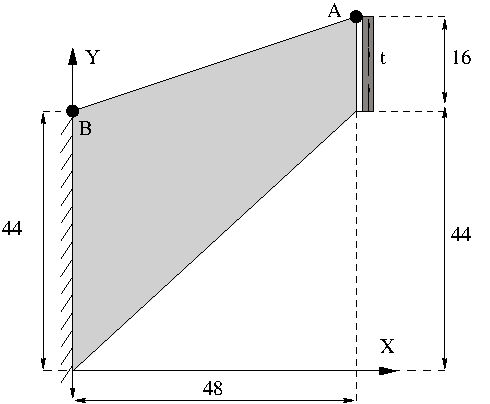
\includegraphics[width=0.9\textwidth]{fig/ue6_cm_problem_description.pdf}
 \captionof{figure}{Cook's Membran Geometrie}\smallskip
Materialparameter:
$E = 210000\,\mbox{MPa} \,,\; \nu = 0.3$

Neumann-Randbedingung:
$t = 5000\,\mbox{MPa}$
\end{minipage}

\enab
  \item Berechnen Sie die Verschiebung in Vertikalrichtung im Punkt $\tt A$ für die verschiedenen Netzverfeinerungsstufen 1)-5) und Veranschaulichen Sie die Ergebnisse in einem ensprechenden Diagramm.

  \textit{Hinweis:} Speichern Sie dazu die jeweiligen Berechnungsergebnisse in der Datei \verb| u-nelem.dat| und nutzen Sie das beigefügte Gnuplot-Skript \verb| u-nelem.gnu|.
 % 
  \item Erzeugen Sie die folgenden Plots
  \begin{itemize}
    \item Netz im Ausgangszustand mit Dirichiet- und Neumann Randbedingungen basierend auf Netzverfeinerungsstufe 2),
    \item Geometrie im Verformten Zustand mit den Spannungs-Contourplots $\sigma_{11}, \sigma_{22}, \sigma_{33}$ basierend auf Netzverfeinerungsstufe 5).
  \end{itemize}
\enae


% \clearpage
% 
% \begin{figure}[h]
% 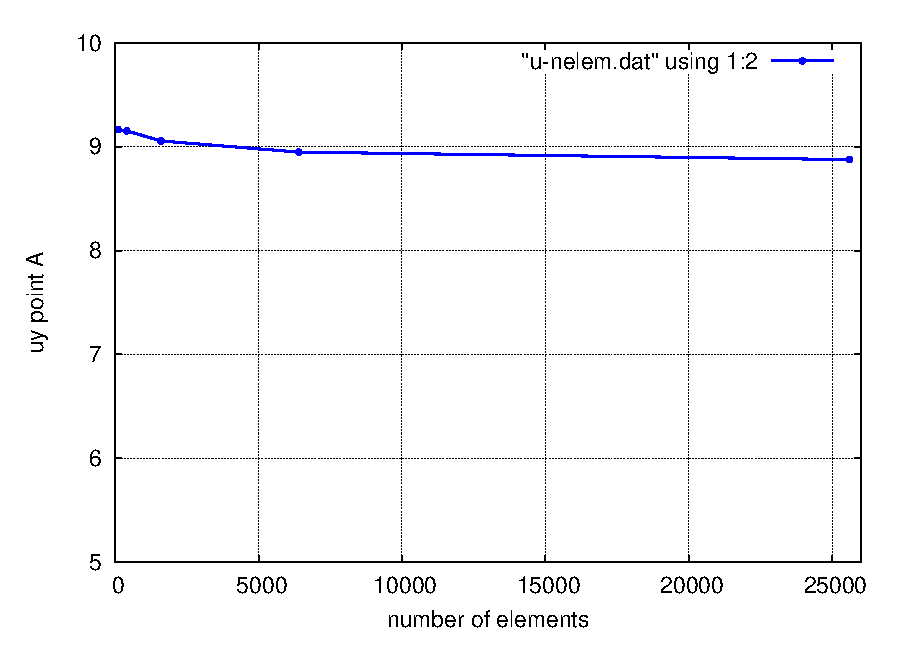
\includegraphics[width=0.9\textwidth]{fig/ue6_u-nelem.eps}
% \caption{Verschiebung im Punkt {\sf A} basierend auf Verfeinerung 1) - 5)}
% \end{figure}
% \begin{figure}[h]
% \includegraphics[width=0.9\textwidth]{mesh_bounds_loads.eps}\\
% \caption{Undeformed mesh (discretization 2) with boundary conditions and applied loads.}
% \end{figure}
% 
% \clearpage
% 
% \begin{figure}[h]
% \centering
% 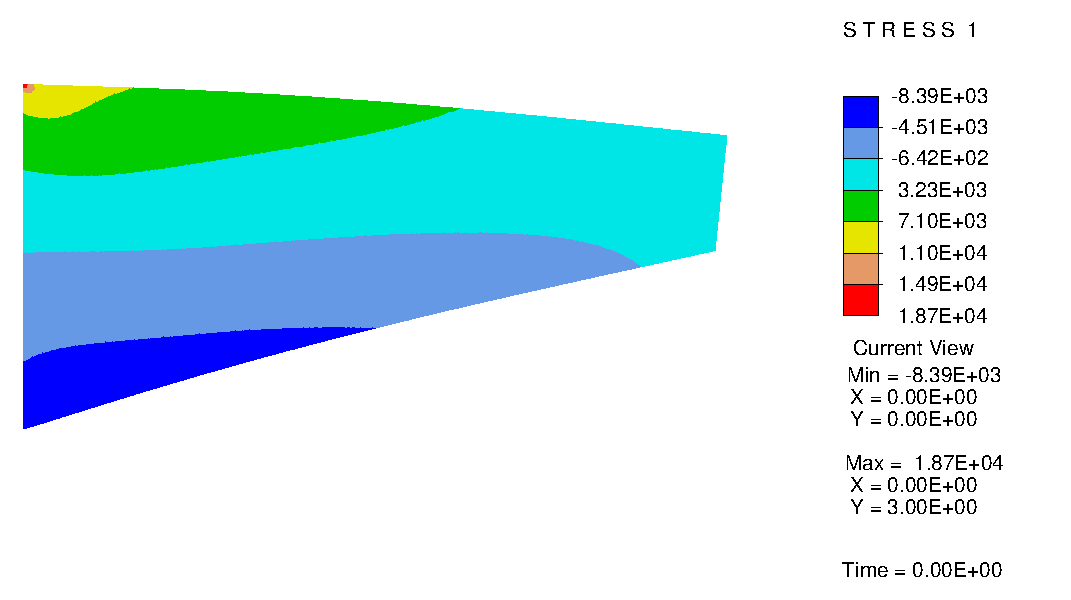
\includegraphics[height=0.32\textheight]{stress11.eps}\\[5mm]
% 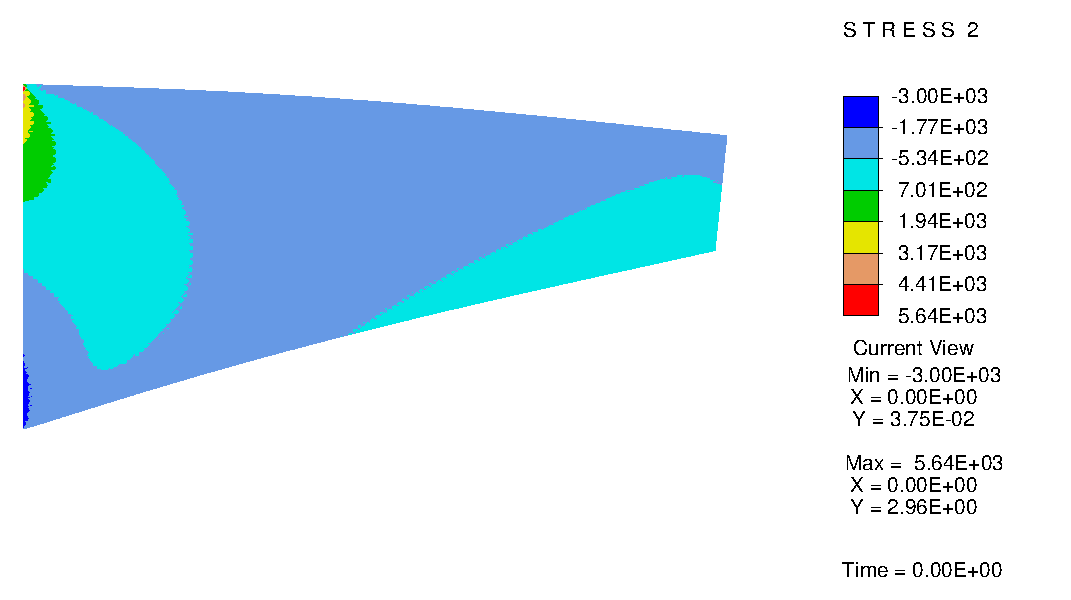
\includegraphics[height=0.32\textheight]{stress22.eps}\\[5mm]
% 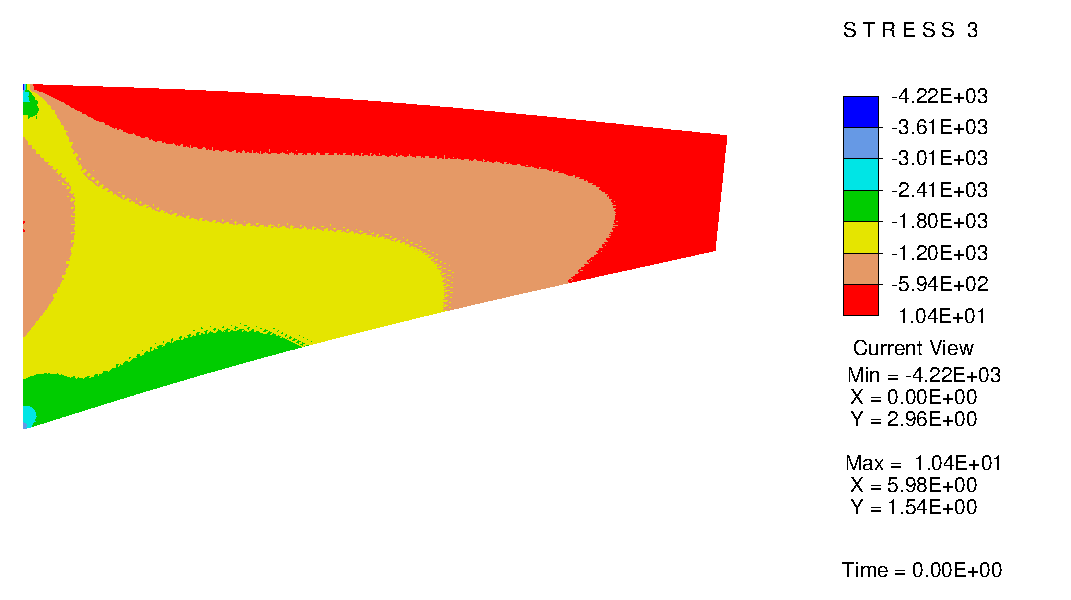
\includegraphics[height=0.32\textheight]{stress33.eps}
% \caption{Stress distributions $\sigma_{11}, \sigma_{22}, \sigma_{33}$}
% \end{figure}

 % einführung feappv
%
%   \setcounter{section}{6}
\clearpage
\setcounter{page}{1}

\section{Lineares Dreieckselement}

Ziel dieser Übung ist es die benutzereigene FEAPpv Elementsubroutine \verb|elmt03| für lineare Dreieckselemente zu erstellen und in das Programm einzubinden.
Dazu werden in den Teilaufgaben stückweise die Unter-Subroutinen erstellt, mithilfe derer schließlich die Elementsteifigkeitsmatrix des linearen Verschiebungs-Dreieckselementes erzeugt wird.



\subsection*{Kompilieren und Ausführen von Fortran Programmen}

Zum Kompilieren und Ausführen der Beispielhaften Fortran Datei $\tt hello\_world.f $ werden auf dem CIP-Pool Rechner folgende Schritte durchgeführt

\begin{enumerate}[label=\arabic*.)]
 \item den bereitgestellten Ordner $\tt ue07\_f$ im persönlichen Laufwerk Z ablegen %(sollte $\tt /cygdrive/z/$ einen Ordner (z.B. $\tt uebung07$) erstellen
 \item unter alle Programme/Cygwin-X auf \enquote{XWin Server} klicken und im Anschluss durch Rechtsklick auf das Cygwin"=Symbol in der Taskleiste unter Systemwerkzeuge ein Cygwin"=Terminal starten,
 \item mit dem Befehl \verb|cd /cygdrive/z/ue07_f| in den Ordner \verb|ue7_f| navigieren
 \item in der Konsole \verb|gfortran -o hello_world hello_world.f| eingeben. 
 Mit diesem Aufruf wird dem Compiler \verb|gfortran| der Befehl gegeben die ausführbare Datei \verb|hello_world| aus dem Fortran-Quellcode der Datei \verb|hello_world.f| zu kompilieren.
 \item in der Konsole \verb|./hello_world| eingeben um das Progamm auszuführen.
 \item[]
 (ggf. muss bei Windows-Systemen bei den Kommandozeileneingaben die Endung \verb|.exe| bei \verb|gfortran| und \verb|hello_world| hinzugefügt werden.)
\end{enumerate}

Schritte 4 und 5 lassen sich auf jeden Fortran Quellcode \verb|<filename>.f| anwenden.\medskip


\clearpage
\subsection*{Hinweise zum Programmieren mit Fortran}

Zur Programmierung k\"onnen nur die Spalten $6-72$ verwendet werden.\\

% \begin{table}
\begin{tabular}{p{60mm}p{70mm}}
%
\textbf{Befehl}                               & \textbf{Wirkung} \\
%
\midrule
\verb|programm <program name>|\newline
...\newline
...\newline
\verb|end program|                            & erste und letzte Zeile eines Programms\\
%
\midrule
\verb|integer i|\newline
\verb|real*8 a|\newline
\verb|real*8 b(10)|                           & Initialisierung von der Variablen i als Integer, a als reelle Zahl und b als Array mit 10 reellen Einträgen \\
%
\midrule
\verb|do i=1,100|\newline
...\newline
...\newline
\verb|end do|                                 & Schleife, in der die Variable i von 1 bis 100 iteriert wird.\\
%
\midrule
\verb|if(r.lt.0)then|\newline
... \verb|Block A| ...\newline
\verb|else|\newline
... \verb|Block B|...\newline
\verb|end if|                                & \enquote{wenn, dann}-Abfrage; hier: wenn r kleiner als 0 ist, wird Block A ausgeführt, ansonsten Block B \\
 \midrule
% \verb|open(1,file='eps_sig.dat')|\newline
% ...\newline
% \verb|write(1,*)'Hello World'|\newline
% ...\newline
% \verb|close(1)| & Öffnen, beschreiben und schließen einer Datei namens \enquote{eps\underline{ }sig.dat} auf unit 1\\
% \hline
\end{tabular}
% \end{table}



\clearpage

\subsection{Berechnen der Elastizitätsmatrix}

Zur Berechnung der Spannungskomponenten in der x-y-Ebene lautet die Elastizitätsmatrix $\mIC^{(V)}$ in Voigt-Notation:

\eb
\mIC=
\begin{bmatrix}
  \lambda + 2\,\mu & \lambda            & 0\\
  \lambda          & \lambda + 2\,\mu  & 0\\
   0              &   0                & \mu
\end{bmatrix}
\ee

Vervollständigen Sie in der Datei \verb|elmt03.f| die Subroutine \verb|dmat03|, sodass mithilfe der Eingabeparameter {\tt yo} (E-Modul) und {\tt nu} (Querkontraktionszahl) die einzelnen Komponenten der Elastizitätsmatrix {\tt aa} berechnet werden.\medskip

\textit{Hinweis:} Um die in dieser und in den folgenden Aufgaben erzeugten Subroutinen zu testen kann die Datei $\tt t1\_test.f$ verwendet werden.
Diese beinhaltet einen Parametersatz (\verb|t1_param|) für ein beispielhaftes Dreieckselement (vgl. Abbildung \ref{fig:t1exam}) und gibt die mit den Subroutinen berechneten Ergebnisse in der Konsole aus (\verb|t1_output_formats|)

{\center
\begin{minipage}{0.46\textwidth}
\center\input{fig/ue7_t1_example.pdf_tex}
\end{minipage}
\begin{minipage}{0.46\textwidth}
\begin{tabular}{ll}
%   \multicolumn{2}{c}{Parameter}\\
\toprule
 E      & $10000$ MPa \\
 $\nu$  & $0.3$ \\
 $x_1,y_1$ &  $0.0, 0.0$ mm \\
 $x_2,y_2$ &  $1.0, 0.3$ mm \\
 $x_3,y_3$ &  $0.5, 0.8$ mm \\
\midrule
\end{tabular}
\end{minipage}
\captionof{figure}{Knotenkoordinaten und Elastizitätsparameter eines Beispielelementes}
\label{fig:t1exam}}





\subsection{Berechnen der B-Matrix}

Die sogennante B-Matrix $\mB^{\mrm{e}}$ hat für das lineare Dreieckselement die Form

\eb
\mB^{\mrm{e}}=
\begin{bmatrix}
 N_{1,x}  & 0        & N_{2,x}  & 0        & N_{3,x}  & 0  \\
 0        & N_{1,y}  & 0        & N_{2,y}  & 0        & N_{3,y}  \\
 N_{1,y}  & N_{1,x}  & N_{2,y}  & N_{2,x}  & N_{3,y}  & N_{3,x}
\end{bmatrix},
\ee

wobei die Ableitungen der Ansatzfunktionen $N_{I}$ für $I\in\{1,2,3\}$ nach den physikalischen Koordinaten mit folgender Formel aufgestellt werden:

\eb
\begin{bmatrix}
 N_{1,x} \\ N_{2,x} \\ N_{3,x}
\end{bmatrix}= \frac{1}{2 A^{\mrm{e}}}
\begin{bmatrix}
 y_2-y_3 \\ y_3-y_1 \\ y_1-y_2
\end{bmatrix}, \qquad
\begin{bmatrix}
 N_{1,y} \\ N_{2,y} \\ N_{3,y}
\end{bmatrix}= \frac{1}{2 A^{\mrm{e}}}
\begin{bmatrix}
 x_3-x_2 \\ x_1-x_3 \\ x_2-x_1
\end{bmatrix}
\ee

Dabei stellt $A^{\mrm{e}}$ die Elementfläche dar, welche sich mithilfe der Determinante der Transformationsmatrix $\mA^{\mrm{e}}$ berechnen lässt:

\eb
2 A^{\mrm{e}} = \det{\mA^{\mrm{e}}} = (x_2-x_1)(y_3-y_1)+(x_3-x_1)(y_1-y_2) \quad\text{mit}\quad
\mA^{\mrm{e}} = \begin{bmatrix}
       1   & 1   & 1   \\
       x_1 & x_2 & x_3 \\
       y_1 & y_2 & y_3
      \end{bmatrix}
\ee

Vervollständigen Sie in der Datei \verb|elmt03.f| die Subroutine \verb|bmat03|, sodass mithilfe der Eingabeparameter \verb|det| (Elementfläche $2 A^{\mrm{e}}$) und \verb|xl| (Knotenkoordinatenmatrix $[2 \times 3]$) die einzelnen Komponenten der B-Matrix {\tt bmat} berechnet werden.


\subsection{Elementsteifigkeitsmatrix aufstellen}

Für lineare Dreieckselemente lässt sich die Elementsteifigkeitsmatrix $\mk^{\mrm{e}}$ wie folgt berechnen:

\eb
\begin{split}
\mk^e&=
\int_{\B^{\mrm{e}}} (\mB^{\mrm{e}})^T \mIC \mB^{\mrm{e}}\ \mrm{d}V =
A^{\mrm{e}}(\mB^{\mrm{e}})^T \mIC \mB^{\mrm{e}}\\ 
% \quad\text{da } \mB^{\mrm{e}}=const.\\
[6\times 6] &= [6 \times 3][3\times 3][3\times 6]
\end{split}
\ee

Hierzu sei eine Scheibendicke von $h$=1 mm angenommen.
Vervollständigen Sie in der Datei \verb|elmt03.f| die Subroutine \verb|kemat03|, sodass mithilfe der Eingabeparameter \verb|bmat| (B-Matrix), \verb|aa| (Elastizitätsmatrix), \verb|det| ($2 A^{\mrm{e}}$) und \verb|nst| (Dimension von $\mk^{\mrm{e}}$) die einzelnen Komponenten der Elementsteifigkeitsmatrix {\tt s} berechnet werden.\medskip

\textit{Hinweis:} Anders als bei \matl\ (vgl. Übung 5) werden Matrix-Multiplikationen in Fortran nicht automatisch durchgeführt. 
Die einzelnen Komponenten des resultierenden Matrixproduktes müssen per Schleifendurchlauf berechnet werden.
Dazu bietet sich an die jeweiligen Matrixmultiplikationen schrittweise zu berechnen und zunächst das Zwischenprodukt

\ebn
\verb|btc| \defeq (\mB^{\mrm{e}})^T \mIC
\een

auszurechnen, mithilfe dessen daraufhin 

\ebn
\verb|s| \defeq A^{\mrm{e}} (\verb|btc|) \mB^{\mrm{e}}
\een

berechnet werden kann.

\clearpage
\subsection{Einbinden in FEAPpv und Beispielrechnung\label{subsec:t1feap}}

\enab
\item Vervollständigen Sie die Elementsubroutine \verb|elmt03| indem sie die aus den voherigen Teilaufgaben aufgestellten Unter-Subroutinen nacheinander aufrufen um die Elementsteifigkeitsmatrix aufzustellen.
\item Ersetzen Sie die nun vervollständigte Datei \verb|elmt03.f| in dem Dateipfad \verb|$FEAPPVHOME4_1/user| und updaten Sie das FEAPpv-Hauptprogram mit dem Befehl \verb|make|.

(Eventuell ist es notwendig die in dem Verzeichnis befindliche Datei \verb|elmt03.f| dem \verb|$FEAPPVHOME4_1/user|-Dateipfad einmal zu öffnen und zu speichern.)
\item Führen die Cook's Membrane-Problem Rechnung (Input-Datei: $\tt I\_cm$) für einen der Netzverfeinerungzustände aus Aufgabe 6.1a) mit dem soeben erstellten User-Element durch und vergleichen Sie die Lösungen.
\enae

\textit{Hinweis:} Benutzerdefinierte Elemente werden in der FEAPpv Inputdatei durch den Befehl

\begin{verbatim}
mate <number>
  user, <user elmt number>
  <user mat par1>  <user mat par2> ...
\end{verbatim}

aufgerufen.
In dem hier vorliegenden Fall sollten die Ergebnisse des implementierten User-Elementes

\begin{verbatim}
mate 1
  user, 3
  E nu
\end{verbatim}

mit denen des in der vorherigen Aufgabe verwendeten programmeigenen linearen Dreieckselementes 

\begin{verbatim}
mate 1
  soli
  elas isot E nu  
\end{verbatim}

mit den Initialisierungsgrößen $\tt \{ndm,nen\}=\{2,3\}$ übereinstimmen.
 % lineares dreieckselement
%
%  \setcounter{section}{7}
\clearpage
\setcounter{page}{1}

\section{Ansatzfunktionen}


\subsection{Verständnisfragen}

\enab
\item Wie lassen sich grundsätzlich FE-Elementansatzfunktionen bestimmen?
\item Welche Eigenschaft der Ansatzfunktionen wird dabei genutzt?
\item Was ist die Idee des isoparametrischen Konzeptes? 
\item Welche Vorteile hat es die FE-Approximation über das Referenzelement im Parameterraum durchuführen?
\enae

\subsection{Isoparametrisches Viereckselement}


{\center\begin{minipage}[t]{0.36\textwidth}
\input{fig/ue8_q1.pdf_tex}
\end{minipage}
\begin{minipage}[t]{0.36\textwidth}
\input{fig/ue8_q2.pdf_tex}
\end{minipage}
\captionof{figure}{lineares und quadratisches Referenzviereckselement im Parameterraum}
\label{fig:qiso}
}

\enab
\item Bestimmen Sie die Ansatzfunktionen $N_1$ und $N_2$ für das lineare Viereckselement aus Abbildung \ref{fig:qiso}
\item Bestimmen Sie die Ansatzfunktionen $N_2$ und $N_6$ für das quadratische Viereckselement aus Abbildung \ref{fig:qiso}
\enae


\clearpage
\subsection{Referenzdreieckselement}


{\center\begin{minipage}[t]{0.36\textwidth}
\input{fig/ue8_p1.pdf_tex}
\end{minipage}
\begin{minipage}[t]{0.36\textwidth}
\input{fig/ue8_p2.pdf_tex}
\end{minipage}
\captionof{figure}{lineares und quadratisches Referenzdreieckselement im Parameterraum}
\label{fig:piso}
}


\enab
\item Bestimmen Sie die Ansatzfunktionen für das lineare Dreieckselement aus Abbildung \ref{fig:piso} mithilfe des allgemeinen Ansatzes
\item Wie lauten die Ansatzfunktionen $N_1$ und $N_6$ für das quadratische Dreieckselement aus Abbildung \ref{fig:piso}. ?
\item Wie lauten die Ansatzfunktionen für ein dreidimensionales lineares Tetraederelement?
\enae % ansatzfunktionen
%
%  \setcounter{section}{8}
\clearpage
\setcounter{page}{1}

\section{Quadratisches Dreieckselement}


In dieser Übung wird die FEAPpv Elementsubroutine \verb|elmt04| für isoparametrische lineare und quadratische Dreieckselemente vervollständigt. 
Ziel ist es insbesondere die Einträge der B-matrix ($N_{I,x}, N_{I,y}$) zu berechnen mithilfe  der kinematischen Beziehungen zwischen Parameter- und physikalischen Koordinaten (Jacobimatrix $\mJ$, Jacobi-Determinante $\det \mJ$ und Inverse der Jacobimatrix $\mJ^{-1}$).


{\center\begin{minipage}{0.36\textwidth}
\input{fig/ue8_p2.pdf_tex}
\end{minipage}
\begin{minipage}{0.36\textwidth}
\center\input{fig/ue9_t2_example.pdf_tex}
\end{minipage}
\captionof{figure}{Quadratisches Referenzdreieckselement im Parameterraum und Beispielement im physikalischen Raum}
\label{fig:p2isph}
}




\subsection{Ableitung der Ansatzfunktionen}


Die Ansatzfunktionen des quadratischen Dreieckselementes lauten 

\eb
\begin{bmatrix}
 N_1 \\ N_2 \\ N_3 \\ N_4 \\ N_5 \\ N_6
\end{bmatrix}=
\begin{bmatrix}
 \lambda_1 ( 2 \lambda_1 - 1) \\ \lambda_2 ( 2 \lambda_2 - 1) \\ \lambda_3 ( 2 \lambda_3 - 1) \\
 4 \lambda_1 \lambda_2 \\ 4 \lambda_2 \lambda_3 \\ 4 \lambda_3 \lambda_1
\end{bmatrix},\quad\text{wobei sich die Flächenkoordinaten mit}\quad
\begin{bmatrix}
 \lambda_1 \\ \lambda_2 \\ \lambda_3
\end{bmatrix}=
\begin{bmatrix}
 \xi \\ \eta \\ 1-\xi-\eta 
\end{bmatrix}
\ee
durch die Parameterkoordinaten $\xi$ und $\eta$ ausdrücken lassen.
Mithilfe der Ableitungen der Ansatzfunktionen nach den Parameterkoordinaten und den physikalischen Knotenkoordinaten lässt sich mithilfe des isoparametrischen Konzeptes die Jacobimatrix

\eb
\mJ = \sum_{I=1}^{\mrm{nen}}
\begin{bmatrix}
 x_I N_{I,\xi}   &  x_I N_{I,\eta}   \\
 y_I N_{I,\xi}   &  y_I N_{I,\eta}
\end{bmatrix}=
\begin{bmatrix}
 x_1 & x_2 & \hdots & x_{\mrm{nen}}  \\
 y_1 & y_2 & \hdots & y_{\mrm{nen}}
\end{bmatrix}
\begin{bmatrix}
 N_{1,\xi} & N_{1,\eta} \\
 N_{2,\xi} & N_{2,\eta} \\
 \vdots    & \vdots     \\
 N_{\mrm{nen},\xi} & N_{\mrm{nen},\eta}
\end{bmatrix}
\label{eq:jacmat}
\ee



aufstellen. 
In der Datei \verb|elmt04.f| in der Subroutine \verb|shape04| wird die Koordinatenmatrix mit \verb|xl| und die Matrix bestehend aus Ableitungen der Ansatzfunktionen nach Parameterkoordinaten mit \verb|sh0| bezeichnet.
\eqref{eq:jacmat} wird demzufolge berechnent durch \verb|xl|.\verb|sh0|$^T$.


\enab
\item Implementieren Sie \eqref{eq:jacmat} zum Aufstellen der Jacobimatrix in der Subroutine \verb|shape04|.
\enae

Zur Berechnung der Ableitung der Ansatzfunktionen nach den physikalischen Koordinaten wird die Inverse der Jacobimatrix benötigt.
Diese lässt sich im 2D-Fall direkt berechnen mit:

\eb
\mJ^{-1}=\frac{1}{\det \mJ} 
\begin{bmatrix}
 \ J_{22}   & - J_{12} \\
 - J_{21}   & \ J_{11}
\end{bmatrix}
\ee

\enabres
\item Ergänzen Sie \verb|shape04| um die Jacobideterminante und die Inverse der Jacobimatrix.
\enae

Die Ableitungen der Ansatzfunktionen lassen sich mit

\eb
\begin{bmatrix}
 N_{I,x} \\ N_{I,y} 
\end{bmatrix}= \mJ^{-T}
\begin{bmatrix}
  N_{I,\xi} \\ N_{I,\eta}
\end{bmatrix}
\ee

durch das folgende Matrixprodukt aufstellen:

\eb
\begin{bmatrix}
 N_{1,x} & \hdots & N_{\mrm{nen},x} \\
 N_{1,y} & \hdots & N_{\mrm{nen},y}
\end{bmatrix}\defeq
\begin{bmatrix}
 \verb|shp(1,*)| \\ \verb|shp(2,*)|
\end{bmatrix}
=\mJ^{-T}.\verb|sh0|
\label{eq:dNidx}
\ee

\enabres
 \item Vervollständigen Sie \verb|shape04| durch die Berechnung der Ableitungen \eqref{eq:dNidx}
\enae


\textit{Hinweis:} Wie in Übung 7 kann die Datei $\tt t2\_test.f$ verwendet werden um die Datei \verb|elmt04.f| zu testen.
Der zur Tabelle \ref{tab:p2para} gehörige Parametersatz für ein entsprechendes Beispielelement befindet sich in der Datei \verb|t2_param|.% und die Ausgabebefehle in der Datei \verb|t2_output_formats|.



{\center
\begin{tabular}{ll|ll}
%   \multicolumn{2}{c}{Parameter}\\
\toprule 
 E      & \multicolumn{3}{l}{$10000$ MPa} \\
 $\nu$  & \multicolumn{3}{l}{$0.3$}  \\
 $x_1,y_1$ &  $0.0, 0.0$ mm & $x_4,y_4$ &  $0.50, 0.15$ mm \\
 $x_2,y_2$ &  $1.0, 0.3$ mm & $x_5,y_5$ &  $0.75, 0.55$ mm \\
 $x_3,y_3$ &  $0.5, 0.8$ mm & $x_6,y_6$ &  $0.25, 0.40$ mm \\
\midrule
\end{tabular}
\captionof{table}{Parameter des quadratischen Dreiecks-Beispielelementes}
\label{tab:p2para}
}


\clearpage
\subsection{Konvergenzstudie}

\enab
\item Ersetzen Sie die vervollständigte Datei \verb|elmt04.f| in dem Dateipfad \verb|$FEAPPVHOME4_1/user| und updaten Sie das FEAPpv-Hauptprogram mit dem Befehl \verb|make|
(vgl Aufgabe 7.4).%\ref{subsec:t1feap})
\item Führen Sie eine Beispielrechnung mit dem linearen und quadratischen User-Element \verb|elmt04.f| durch und vergleichen sie die Lösungen mit denen der entsprechenden programmeigenenen Dreieckselemente.
\item Führen Sie die Netzkonvergenzstudie aus Aufgabe 6.1a) für das quadratische Dreieckselement durch und vergleichen Sie die Ergebnisse mit denen des linearen Dreieckselementes. 
Welcher der beiden Elementtypen hat hier ein vorteilhafteres Konvergenzverhalten?
\enae
 % quadratisches dreieckselement
%
% \setcounter{section}{9}
\clearpage
\setcounter{page}{1}

\section{Vierknotenelement}

In dieser Übung wird die FEAPpv Elementsubroutine \verb|elmt04| aus den vorherigen Aufgaben um das isoparametrische Vierknotenelement (vgl. Abbildung \ref{fig:q1gp}) erweitert.

{\center
\input{fig/ue10_q1.pdf_tex}
\captionof{figure}{lineares Referenzviereckselement mit Gausspunkten}
\label{fig:q1gp}
}\medskip

\textbf{Grundlagen:}
Mithilfe der Gausspunkte wird das Integral der Elementsteifigkeitsmatrix $\mk^{\mrm{e}}$ wie folgt numerisch berechnet: 

\eb
\mk^{\mrm{e}} = \int_{\B^{\mrm{e}}} (\mB^{\mrm{e}})^T \mIC\ \mB^{\mrm{e}}\ \mrm{d}V
 = \sum_{l=1}^{ n_{\mrm{GP}}=4} (\mB^{\mrm{e}}(\Bxi_l))^T \mIC\ \mB^{\mrm{e}}(\Bxi_l) \det\mJ(\Bxi_l) \mrm{w}_l
 \label{eq:q1ke}
\ee

Dabei sind $\Bxi_l=[\xi_l,\eta_l]^T $ die Ortsvektoren der Gausspunkte im Parameterraum und $\mrm{w}_l$ die zugehörigen Wichtungsfaktoren.
Für das Vierknotenelement sind diese Tabelle \ref{tab:q1gp} zu entnehmen.

{\center\begin{tabular}{llll}
%   \multicolumn{2}{c}{Parameter}\\
\toprule
 i      & $\xi_l$ & $\eta_l$ & $\mrm{w}_l$\\\midrule
 1      &   $-1/\sqrt{3}$ &  $-1/\sqrt{3}$ & $1$\\
 2     & $ \ \ 1/\sqrt{3}$ &  $-1/\sqrt{3}$ & $1$\\
 3    & $\ \ 1/\sqrt{3}$ &  $\ \ 1/\sqrt{3}$ & $1$\\
 4    & $ -1/\sqrt{3}$ &  $\ \ 1/\sqrt{3}$ & $1$\\
\midrule
\end{tabular}
\captionof{table}{Gausspunktkoordinaten und Wichtungsfaktoren des Vierknotenelementes}
\label{tab:q1gp}
}\medskip

Die Summe in \eqref{eq:q1ke} wird im FE-Programm üblicherweise im Schleifendurchlauf aufgestellt, wobei $\mk^{\mrm{e}}$ in jedem Iterationsschritt $l$ geupdated wird:

\begin{align*}
 & \mk^{\mrm{e}} = \mk^{\mrm{e}}_0\ (\text{in linear elasticity}= \bzero )&&\\
 & \text{\textbf{do}}\  l=1\ , \  n_{\mrm{GP}}  \\
 & \quad \mk^{\mrm{e}}\Longleftarrow \mk^{\mrm{e}}+ (\mB^{\mrm{e}}(\Bxi_l))^T \mIC\ \mB^{\mrm{e}}(\Bxi_l) \det\mJ(\Bxi_l) \mrm{w}_l \\
 & \text{\textbf{end do}}
\end{align*}



Desweiteren werden im Postprocessing, nachdem das FE-Problem gelöst ist und der Elementverschiebungsvektor $\md^{\mrm{e}}$ bekannt ist, an den Gausspunkten die Spannungen und Verzerrungen ausgewertet.
Mithilfe der aus der Vorlesung bekannten Element-Interpolationsfunkionen $\mN^{\mrm{e}}$ und $\mB^{\mrm{e}}$ kann der Gausspunkt in physikalischen Koordinaten ausgedrückt werden:

\eb
\mx^h(\Bxi_l) = \mN^{\mrm{e}}(\Bxi_l) \mx^{\mrm{e}}
\label{eq:xgp}
\ee

Die Verzerrung, welche diesem Punkt zugeordnet ist lässt sich (in Voigt-Notation) wie folgt bestimmen:

\eb
\Mvarepsilon^{\mrm{V}}(\Bxi_l) = \mB^{\mrm{e}}(\Bxi_l) \md^{\mrm{e}}
\label{eq:ppeps}
\ee

Mithilfe des Elastizitätstensors $\mIC^V$ lässt sich ebenso die Spannung bestimmen:

\eb
\Msigma^{\mrm{V}}(\Bxi_l) = \mIC^V \Mvarepsilon^{\mrm{V}}(\Bxi_l)
\label{eq:ppsig}
\ee
%
\subsection{Gausspunkte}

Die Subroutine \verb|gauss04(l,lint,eg,wg)| gibt die Koordinaten \verb|eg| und Wichtungsfaktoren \verb|wg| bei Input des aktuellen Gausspunktes \verb|l|.
\verb|lint| stellt dabei die Anzahl an Elementgausspunkten dar (lineares Dreieck t1: \verb|lint|=1, quadratisches Dreieck t2: \verb|lint|=3 oder lineares Viereck q1: \verb|lint|=4).
%
\enab
\item Vervollständigen Sie \verb|gauss04| um die Informationen aus Tabelle \ref{tab:q1gp}.
\enae
%
\subsection{Postprocessing}

Die Subroutine \verb|str04| berechnet die Verzerrungen \verb|eps| und Spannungen \verb|sig| aus den Elementknotenverschiebungen \verb|du|.
Dazu werden die Berechnungsschritte \eqref{eq:xgp}-\eqref{eq:ppsig} durchgeführt. 
Die zugehörigen Programmvariablennamen sind Tabelle \ref{tab:ppparam} zu entnehmen.


{\center
\begin{tabular}{llllllll}
%   \multicolumn{2}{c}{Parameter}\\
\toprule
 $\mx^h(\Bxi_l)$                   & 
 $\mN^{\mrm{e}}(\Bxi_l)$           & 
  $\mx^{\mrm{e}}$                  & 
  $\md^{\mrm{e}}$                  &
  $\mB^{\mrm{e}}(\Bxi_l)$          &
 $\Mvarepsilon^{\mrm{V}}(\Bxi_l)$  &
 $\mIC^V$                          &
 $\Msigma^{\mrm{V}}(\Bxi_l)$       \\
  \verb|xg| & \verb|shp(3,*)| & \verb|xl| & \verb|du| & \verb|bmat| & \verb|eps| & \verb|aa|$^*$ & \verb|sig|   
\\\midrule
\end{tabular}
  \captionof{table}{Zuordnung der Programm-Variablennamen zu den Berechnungsgrößen.}
\label{tab:ppparam}
}\medskip

\textit{Hinweis:} 
\verb|aa|$^*$ ist die $[3\times3]$-Elastizitätsmatrix, deren Einträge zur x-y-Ebene gehören.
Da die implementierten Elemente einen ebenen Verzerrungszustand beschreiben ist zu berücksichtigen, dass $\sigma_{33}\neq 0$ zusätzlich zu berechnen ist.

\enab
\item Ergänzen Sie \verb|str04| um die Berechnung \eqref{eq:xgp} der phys. Gausspunktkoordinaten
\item Ergänzen Sie \verb|str04| um die Berechnung \eqref{eq:ppeps} der Verzerrungen
\item Ergänzen Sie \verb|str04| um die Berechnung \eqref{eq:ppsig} der Spannungen
% \item Testen Sie \verb|elmt04.f| mit einer Beispielrechnung (\verb|I_cm|) und Vergleichen Sie Outputdateien und Contourplots mit denen der programmeigenen Elemente
\enae


\clearpage
\subsection{Konvergenzstudie}

\enab
\item Ersetzen Sie die vervollständigte Datei \verb|elmt04.f| in dem Dateipfad \verb|$FEAPPVHOME4_1/user| und updaten Sie das FEAPpv-Hauptprogram mit dem Befehl \verb|make|
(vgl Aufgabe 9.2).%\ref{subsec:t1feap})
\item Testen Sie \verb|elmt04.f| mit einer Beispielrechnung (\verb|I_cm|) und Vergleichen Sie die Ausgabe der Spannungen und Verzerrungen in der Outputdatei (\verb|O_cm|) und die Contourplots mit denen der programmeigenen Elemente.
\item Ergänzen Sie Netzkonvergenzstudie aus Aufgabe 9.2c) mit den Ergebnissen des Viereckselementes.
Plotten Sie die Verschiebung des Eckpunktes \verb|A| über der Anzahl der Freiheitsgrade.
Macht es einen qualitativen unterschied ob der Konvergenzplot über der Anzahl der Freiheitsgrade oder der Anzahl der Elemente erstellt wird? 
\enae


% \subsection{Konvergenzstudie}
% 
% Vergleichen Sie das Konvergenzverhalten des linearen Viereckselementes mit den Elementen aus den vorherigen Aufgaben.
% Lösen Sie Dazu das Cook's Membrane Randwertproblem für verschieden feine Netze und betrachten Sie die Verschiebung am Eckpunkt A (vgl. Aufgabe 6.1a).
 % viereckselement
% %
%  \setcounter{section}{10}
\clearpage
\setcounter{page}{1}

\section{Gauss-Quadratur}

Die Formel für die numerische Integration mittels Gauss-Quadratur lautet
\eb
\int_{-1}^1 f(\xi)\ \mrm{d} \xi \approx
\sum_{i=1}^n w_i\ f(\xi_i)\ .
\ee
Dabei sind $w_i$ die Wichungsfaktoren und $\xi_i$ die Gausspunkte.


\subsection{Quadratisches Viereckselement}

Für das quadratische isoparametrische Viereckselement wird die Gaussintegrationsordnung $n=3$ gewählt.

\enab
\item Wie viele Gausspunkte hat das Element dann? 
\item Ist die Gaussintegration der Ordnung $n=3$ für eine quadratische Funktion $f(\xi)$ (Polynomgrad $p=2$) exakt? 
      Welche Bedingung muss erfüllt sein?
          
      \textit{Hinweis}: Da bei Viereckselementen die Übertragung von einer auf zwei Koordinatenrichtungen direkt möglich ist reicht es in dieser Aufgabe eine Funktion $f(\xi)$ mit nur einer Koordinate zu betrachten.
\enae




\enabres
\item Gibt es Gründe eine höhere Integrationsordnung als nötig zu verwenden? Erläutern Sie ihre Antwort anhand eines Beispiels.
\enae

Findet die Gaussintegration über das Intervall $[-1,1]$ statt so lassen sich die Gausspunke $\xi_i\ (i=1,\hdots,n)$ als Nullstellen des n-ten Legendrepolynoms bestimmen:

\eb
P_n(\xi)=\frac{1}{2^n\,n!}\ \frac{\mrm{d}^n}{\mrm{d}\xi^n}(\xi^2-1)^n
\ee

\enabres
\item Wie lautet das Legendrepolynom 3. Ordnung?
\item Bestimmen Sie die entsprechenden Gausspunktkoordinaten $\xi_i$
\enae

Die Zugehörigen Wichtungsfaktoren $w_i$ lassen sich über folgende Beziehung bestimmen:

\eb
w_i=\int_{-1}^1 l_i(\xi)\ \mrm{d}\xi
\ee

Dabei ist $l_i$ das i-te Lagrangepolynom (Polynomgrad: $n-1$) mit den Gausspunkten $\xi_i$ als Stützstellen.

\enabres
\item Bestimmen Sie die zu den Gausspunktkoordinaten gehörigen Wichtungsfaktoren $w_i$
\enae

\clearpage


% \subsection*{Zusatzinfo: Herleitung Gausspunktbestimmung}

 % numerische integration
% 
% 
\kvlayout
%
\clearpage
\setcounter{page}{1}


\section{Klausurvorbereitung}



\subsection{Schwache Form und Idee der FEM}

Gegeben sei das elastische Potential

\ebn
\varPi = \frac{1}{2} \int_{\B} \Bvarepsilon \cdot \Bsigma\ \mrm{dv} 
- \int_{\B} \bu \cdot \bar{\bb}\ \mrm{dv}
- \int_{\p{}\B_t} \bu \cdot \bar{\bt}\ \mrm{da}
\een

\enab
\item Wie lautet die zugehörige Variationsgleichung (schwache Form)?
\item Leiten Sie aus der schwachen Form die Euler Lagrange-Gleichungen (starke Form) für das Randwertproblem der Elastostatik her.
\item Wie gelangt man von der schwachen Form zur Elementsteifigkeitsmatrix $\mk_e$ und Elementlastmatrix $\mmp_e$?
\item Wie lassen sich die Integrale in der diskretisierten schwachen Form berechnen?
\item Wie gelangt man zur Lösung des globalen Problems?
\enae


\subsection{Assemblierung}

Gegeben sei das in Abbildung \ref{fig:kvassem} dargestellte Mini-Randwertproblem bestehend aus linearen Dreieckselementen. 


{\center
\input{fig/kv_assem.pdf_tex}
\captionof{figure}{}
\label{fig:kvassem}
}

\enab
\item Erstellen Sie eine Skizze, in der alle globalen Knotenfreiheitsgrade (ohne Berücksichtigung der Randbedingungen) eingetragen sind.
\item Wie lauten die Einträge des globalen Lösungsvektors unter Berücksichtigung der Randbedingungen? 
      Wie lautet der globale Lastvektor?
\item Wie lauten die Einträge der Elementsteifigkeitsmatrix $\mk^1$ und $\mk^2$, welche nach Berücksichtigung der Randbedingungen in die globale Steifigkeitsmatrix eingehen?
      Bestimmen Sie die Einträge der globalen Steifigkeitsmatrix $\mK$.
\enae



% \subsection{Lagrange Polynome}


\clearpage
\subsection*{Fragenkatalog}

\subsubsection*{Kontinuumsmechanik}
\begin{itemize}
 \item Was ist die Voigt-Notation? Welche Annahmen ermöglichen es diese zu verwenden?
 \item Wie lautet der Elastizitätstensor in Voigt-Notation?
 \item Was ist der Unterschied zwischen ebenem Verzerrungs- und ebenem Spannungszustand?
 % Aw: annahmen: symmetrie von \varepsilon and \sigma
\end{itemize}



% \subsubsection*{Assemblierung}
% \begin{itemize}
%   \item Assemblierungsaufgabe wie in Übung
% %   \item Wie werden Dirichlet-Randbedingungen in dem globalen Gleichungssystem berücksichtigt?
%  \item Wie werden Neumann-Randbedingungen in dem globalen Gleichungssystem berücksichtigt?
%  \item Grundprozedur FEM
%  \item Welche Informationen stecken in der Elementsteifigkeitsmatrix?
% \end{itemize}



\subsubsection*{Grundkonzept der FEM}
\begin{itemize}
 \item Was sind die grundlegenden Schritte der Finite-Elemente Analyse?
 \item Leiten sie Elementsteifigkeitsmatrix und -lastmatrix her
  \item Wie werden Lagerungen in dem globalen Gleichungssystem berücksichtigt, wie werden die ensprechenden Randbedingungen noch genannt?
  \item Welche zwei verschiedenen Arten von Randbedingungen kennen Sie? Worin unterscheiden sie sich?
  \item Was passiert wenn Randbedingungen weggelassen werden?
  \item Welche verschiedenen Elementtypen kennen Sie?
\end{itemize}


\subsubsection*{Isoparametrisches Konzept}
\begin{itemize}
 \item Wie lauten die Ansatzfunktionen für das bilineare/quadratische Viereckselement? (Aufstellen der zugehörigen Lagrange-Polynome)
 \item Was besagt das Isoparametrische Konzept? Warum wird es verwendet?
 \item Wozu wird die Jacobideterminante benötigt? Wie wird sie bestimmt?
\end{itemize}



\subsubsection*{Numerische Integration}
\begin{itemize}
\item Warum wird die Gauss-Integration benötigt?
\end{itemize}


Gegeben sei ein Polynom $f(\xi)$ mit dem Polynomgrad $n=1/2/3/...$. 
\begin{itemize}
 \item Wieviele Gausspunkte sind erforderlich damit die Integration exakt ist?
 \item Wie lauten die zugehörigen Gausspunkte und Wichtungsfaktoren? (entsprechende Formeln auswerten)
 \item Was passiert wenn eine höhere Integrationsordung als erforderlich verwendet wird?
 \item Wie lauten die Legendre-Polynome der Ordnung $n=1/2/3/...$?
\end{itemize}

\subsubsection*{Konvergenz und Diskretisierungsfehler}

\begin{itemize}
 \item Wie lässt sich das Konvgenzverhalten verschiedener Elemente vergleichen? Skizzieren Sie einen beispielhaften entsprechende Konvergenzplot.
 \item Welche zwei verschiedenen Arten von A-Posteori Fehlerschätzern haben Sie kennengelernt, worin unterscheiden sich diese?
 \item Womit lässt sich die Qualität eines Fehlerschätzers ermitteln?
 \item Wird der Diskretisierungsfehler bei Erhöhung der Elementanzahl für das gleiche Randwertproblem größer oder kleiner? Begründen Sie Ihre Antwort.
 \item Was sind superkonvergente Punkte?
 \item Handelt es sich bei den Verschiebungen $\bu^h$, wenn sie mit Lagrange-Ansatzfunktionen über die Knoten interpoliert um Funktionen, welche zwischen den Elementen kontinuierlich sind? Wie verhält es sich mit den zugehörigen Verzerrungen $\Bvarepsilon^h$? 
 \item An welchen Punkten werden Verzerrungen und Spannungen im Postprocessing üblicherweise ausgewertet und warum?
 \end{itemize}


\subsubsection*{Locking und gemischte Elemente}

\begin{itemize}
 \item Wann spricht man von inkompressiblem Material? Welche Probleme können auftreten?
 \item Was sind die Vorteile gemischter Elemente gegenüber standard Verschiebungselementen?
 \item Wie lautet das Hellinger-Reissner Variationsprinzip?
 \item Wie lautet das Hu-Washizu Variationsprinzip für das Q1P0 element?
\end{itemize}


 % klausurvorbereitung
%


\end{document}
